\documentclass[10pt]{article}

\usepackage[T1]{fontenc}
\usepackage[utf8]{inputenc}
\usepackage{lmodern}
\usepackage{amsmath}
\usepackage{amssymb}
\usepackage{pifont}
\usepackage{bm}
\usepackage{graphicx}
\usepackage[space]{grffile}
\usepackage{multicol}
\usepackage{array}
\usepackage{tabu}
\usepackage{ragged2e}
\usepackage{setspace}
\usepackage{xr}
\usepackage[font=small,labelfont=bf,labelsep=period]{caption}
%\usepackage{subcaption}
%\usepackage[CaptionAfterwards]{fltpage}
\usepackage{subfigure}
\usepackage{lineno}
\linenumbers
\usepackage{tikz}
\def\checkmark{\tikz\fill[scale=0.4](0,.35) -- (.25,0) -- (1,.7) -- (.25,.15) -- cycle;} 
\usepackage[margin=1.0in]{geometry}

\usepackage[backend=biber,style=authoryear,sorting=nyt,url=false,isbn=false,doi=false,firstinits=true]{biblatex}

\DeclareNameAlias{default}{last-first}

\DefineBibliographyStrings{english}{%
	andothers = {\addcomma\addspace\textsc{et\addabbrvspace al}\adddot},
	and = {\textsc{and}}
}
\renewcommand*{\labelnamepunct}{\space\space}

\renewbibmacro{in:}
{%
	\ifentrytype{article}{%
	}{%
		\printtext{\bibstring{in}\intitlepunct}%
	}%
}
\renewbibmacro*{volume+number}{%
	\printfield{volume}%
	\setunit*{\addcomma\space}%
	\printfield{number}%
	\setunit{\addcomma\space}}

\DeclareFieldFormat{pages}{#1}

\renewbibmacro*{publisher+location+date}{%
	\printlist{publisher}%
	\setunit*{\addcomma\space}%
	\setunit*{\addcomma\space}%
	\usebibmacro{date}%
	\newunit}

\renewcommand{\newunitpunct}{\addcomma\space}
\DeclareFieldFormat[article,inbook,incollection,inproceedings,patent,thesis,unpublished]{title}{#1} 
\DeclareFieldFormat{year}{#1} 

\renewcommand{\baselinestretch}{2.0}
\addbibresource{refs/ident_refs.bib}

\renewcommand{\thefigure}{S\arabic{figure}}
\renewcommand{\figurename}{Supplementary Figure}
\renewcommand{\thetable}{S\arabic{table}}
\renewcommand{\tablename}{{Supplementary Table}}

\renewcommand\thesection{S\arabic{section}}
\renewcommand\thesubsection{\thesection.\arabic{subsection}}
\renewcommand{\theequation}{S\arabic{equation}}

\externaldocument{draft_2} % reference to existing external document

\captionsetup{font={stretch=2.0}}
\begin{document}
	\begin{center}
		\begin{Large}
			Manuscript Title 
		\end{Large}\\
		Shyam Srinivasan\textsuperscript{a}, William R. Cluett\textsuperscript{a} and Radhakrishnan Mahadevan\textsuperscript{*,a,b}\\
	\end{center}	
\section{Supplementary Tables}
\begin{table}[!thbp]
	\caption{Table showing the perturbed values of all parameters used to generate experimental data in silico for testing practical identifiability of all fluxes in the small metabolic network.}
	\begin{center}				
		\begin{tabular}{lp{3.5cm}cccccp{2cm}}
			\hline
			Experiment Type & Perturbed Parameter (wild type value a.u.)& \multicolumn{5}{c}{Perturbed Values a.u.} & Number of Experiments\\
			\hline
			wild type &  &\multicolumn{5}{l}{} & 1\\
			acetate perturbation & $acetate$ (0.1) & 0.05 & 0.09 & 0.2 & 0.5 & 1.0 & 5\\
			$v_1$ perturbation & $k_1^{cat}$ (1) & 0.5 & 0.9 & 1.1 & 1.5 & 2.0 & 5\\				
			$v_2$ perturbation & $V_2^{max}$ (1) & 0.5 & 0.9 & 1.1 & 1.5 & 2.0 & 5\\								
			$v_3$ perturbation & $V_3^{max}$ (1) & 0.5 & 0.9 & 1.1 & 1.5 & 2.0 & 5\\
			\hline
			\multicolumn{7}{l}{Total number of experimental data sets used for practical parameter identification:} & 21\\
			\hline
		\end{tabular}
	\end{center}	
	\label{tab:pval}
\end{table}	

\clearpage

\section{Supplementary Figures}	
\begin{figure}[!tbhp]
	\centering{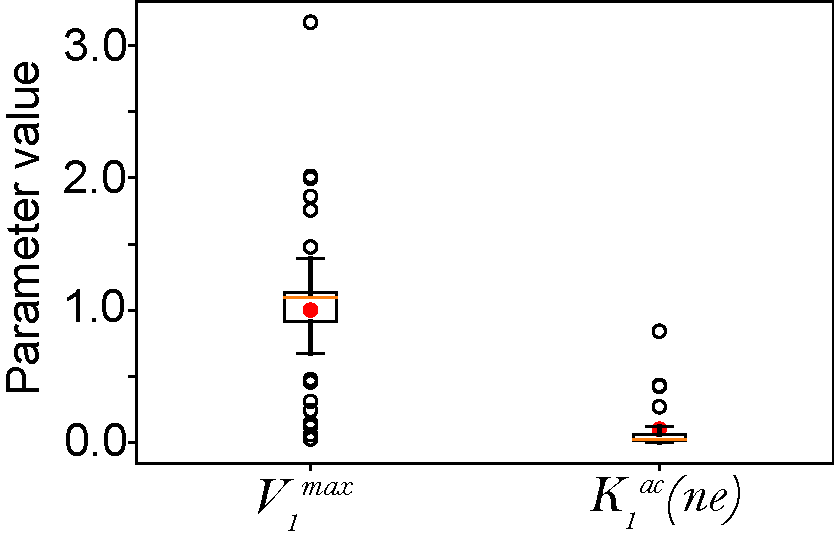
\includegraphics[width=0.6\textwidth,height=0.2\textheight, keepaspectratio]{figures/figure6/v1_v1max_ck_parameter_values}}
	\caption{}\label{fig:v1_v1max_ck_values}
\end{figure}

\begin{figure}[!tbhp]
	\centering{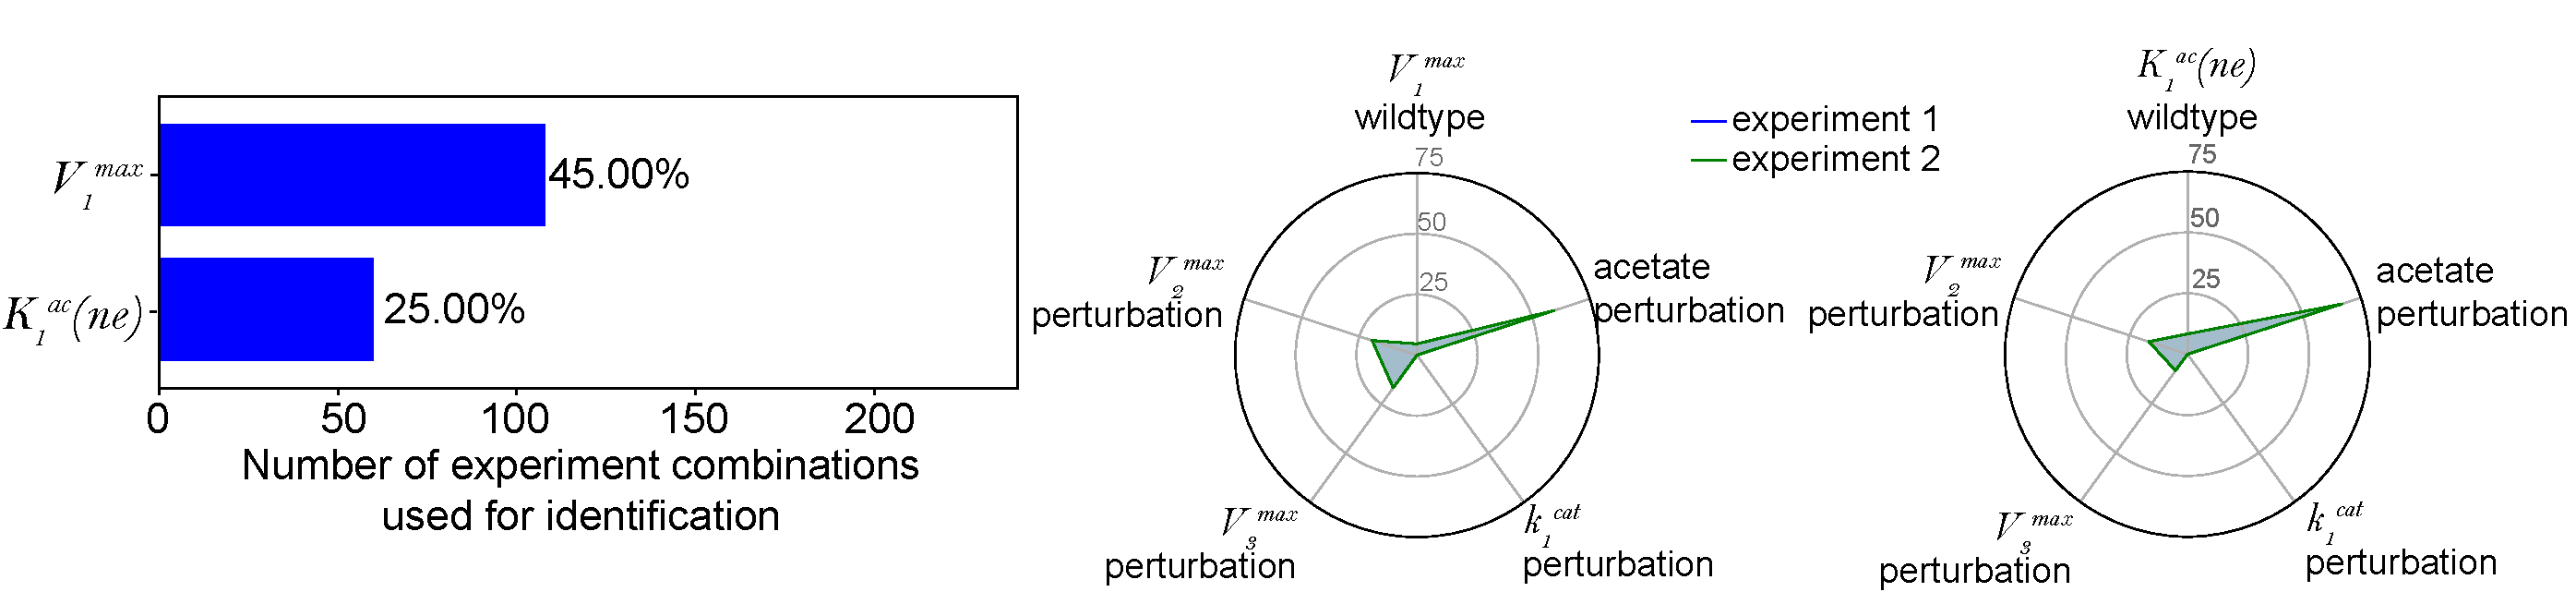
\includegraphics[width=1.0\textwidth,height=0.3\textheight, keepaspectratio]{figures/figure1/v1_v1max_ck_ident_exp_info}}
	\caption{}\label{fig:v1_v1max_ck_ident}
\end{figure}	

\begin{figure}[!tbhp]
	\centering{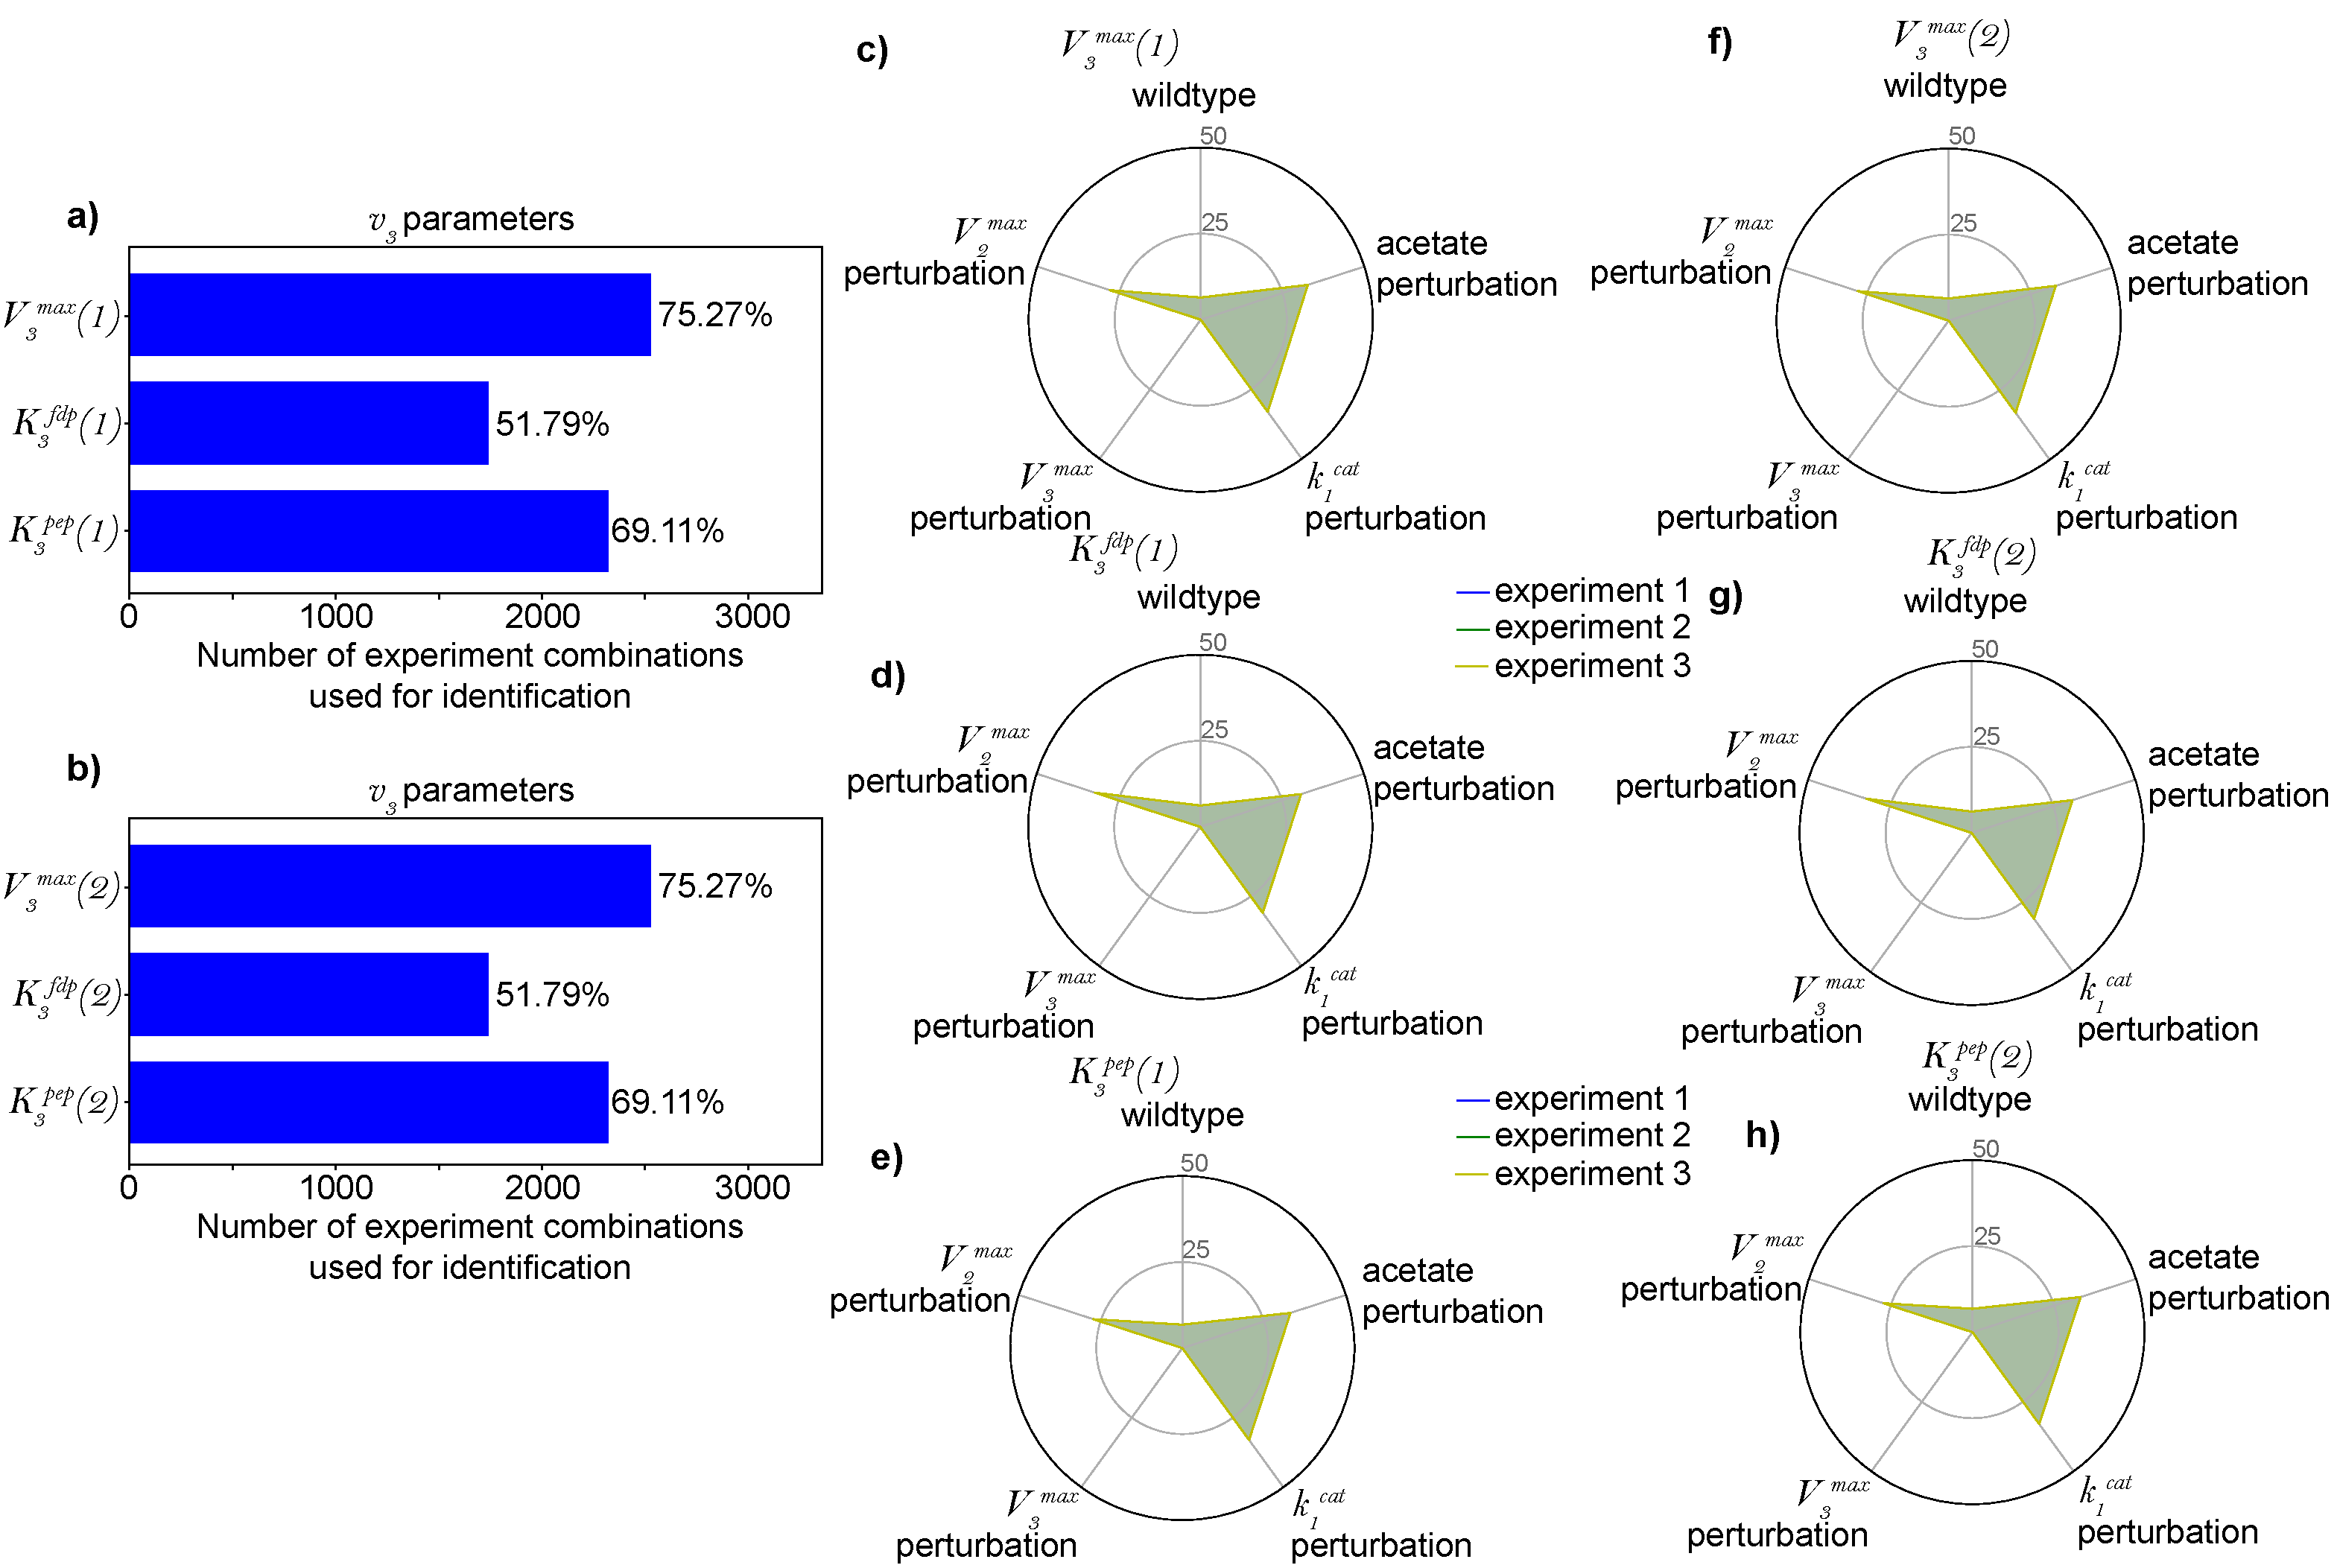
\includegraphics[width=1.0\textwidth,height=0.6\textheight, keepaspectratio]{figures/figure1/v3_ck_1_2_ident_exp_info}}
	\caption{}\label{fig:v3_1_ck_ident}
\end{figure}	

\begin{figure}[!tbhp]
	\centering{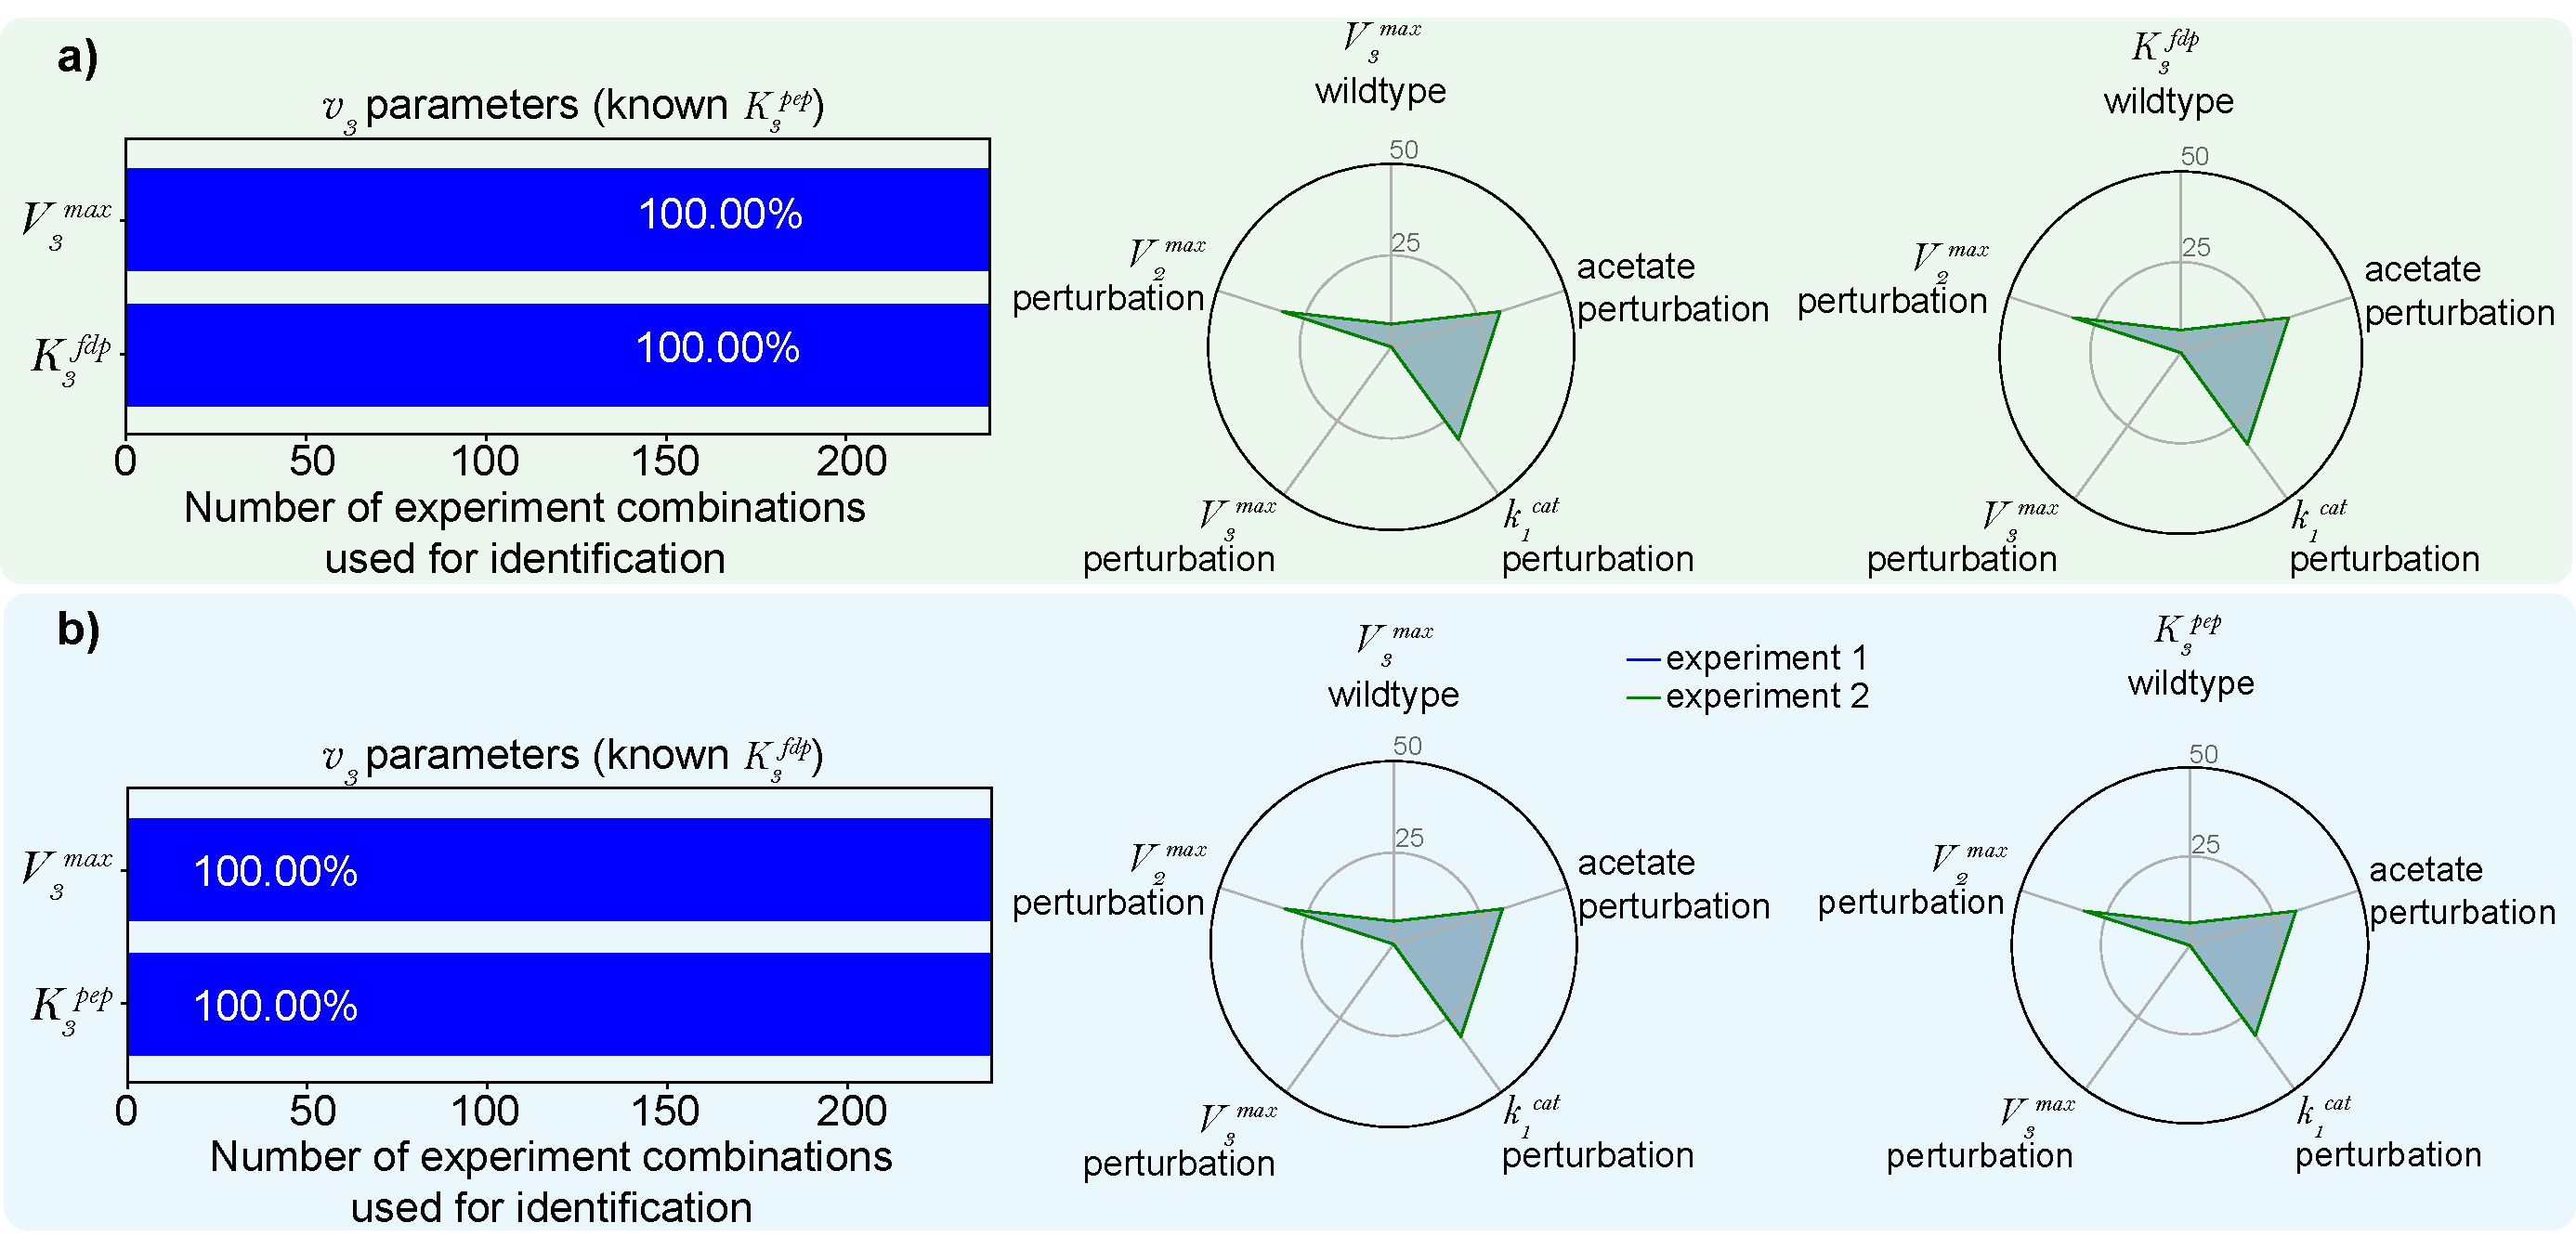
\includegraphics[width=1.0\textwidth,height=0.3\textheight, keepaspectratio]{figures/figure1/v3_var_1_2_ck_ident_exp_info}}
	\caption{}\label{fig:v3_var_1_2_ck_ident}
\end{figure}

\begin{figure}[!tbhp]
	\centering{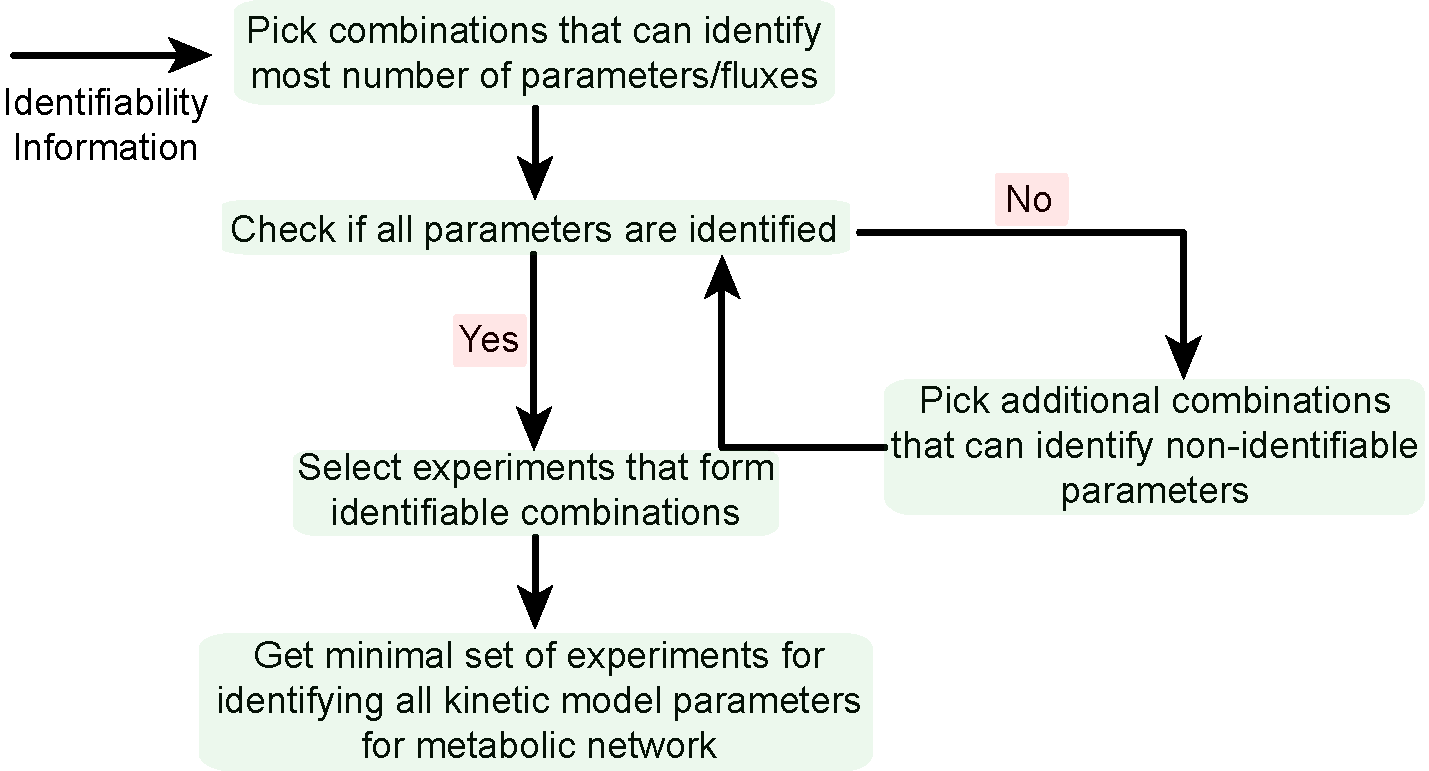
\includegraphics[width=0.6\textwidth,height=0.6\textheight,keepaspectratio]{figures/figure3/experimental_design}}
	\caption{Flow diagram showing a method for experimental design that uses our methodology for practical identification of parameters to determine the number and type of experiments required to identify all fluxes within a given metabolic network.}\label{fig:ident-design}
\end{figure}

\begin{figure}[!tbhp]
	\centering{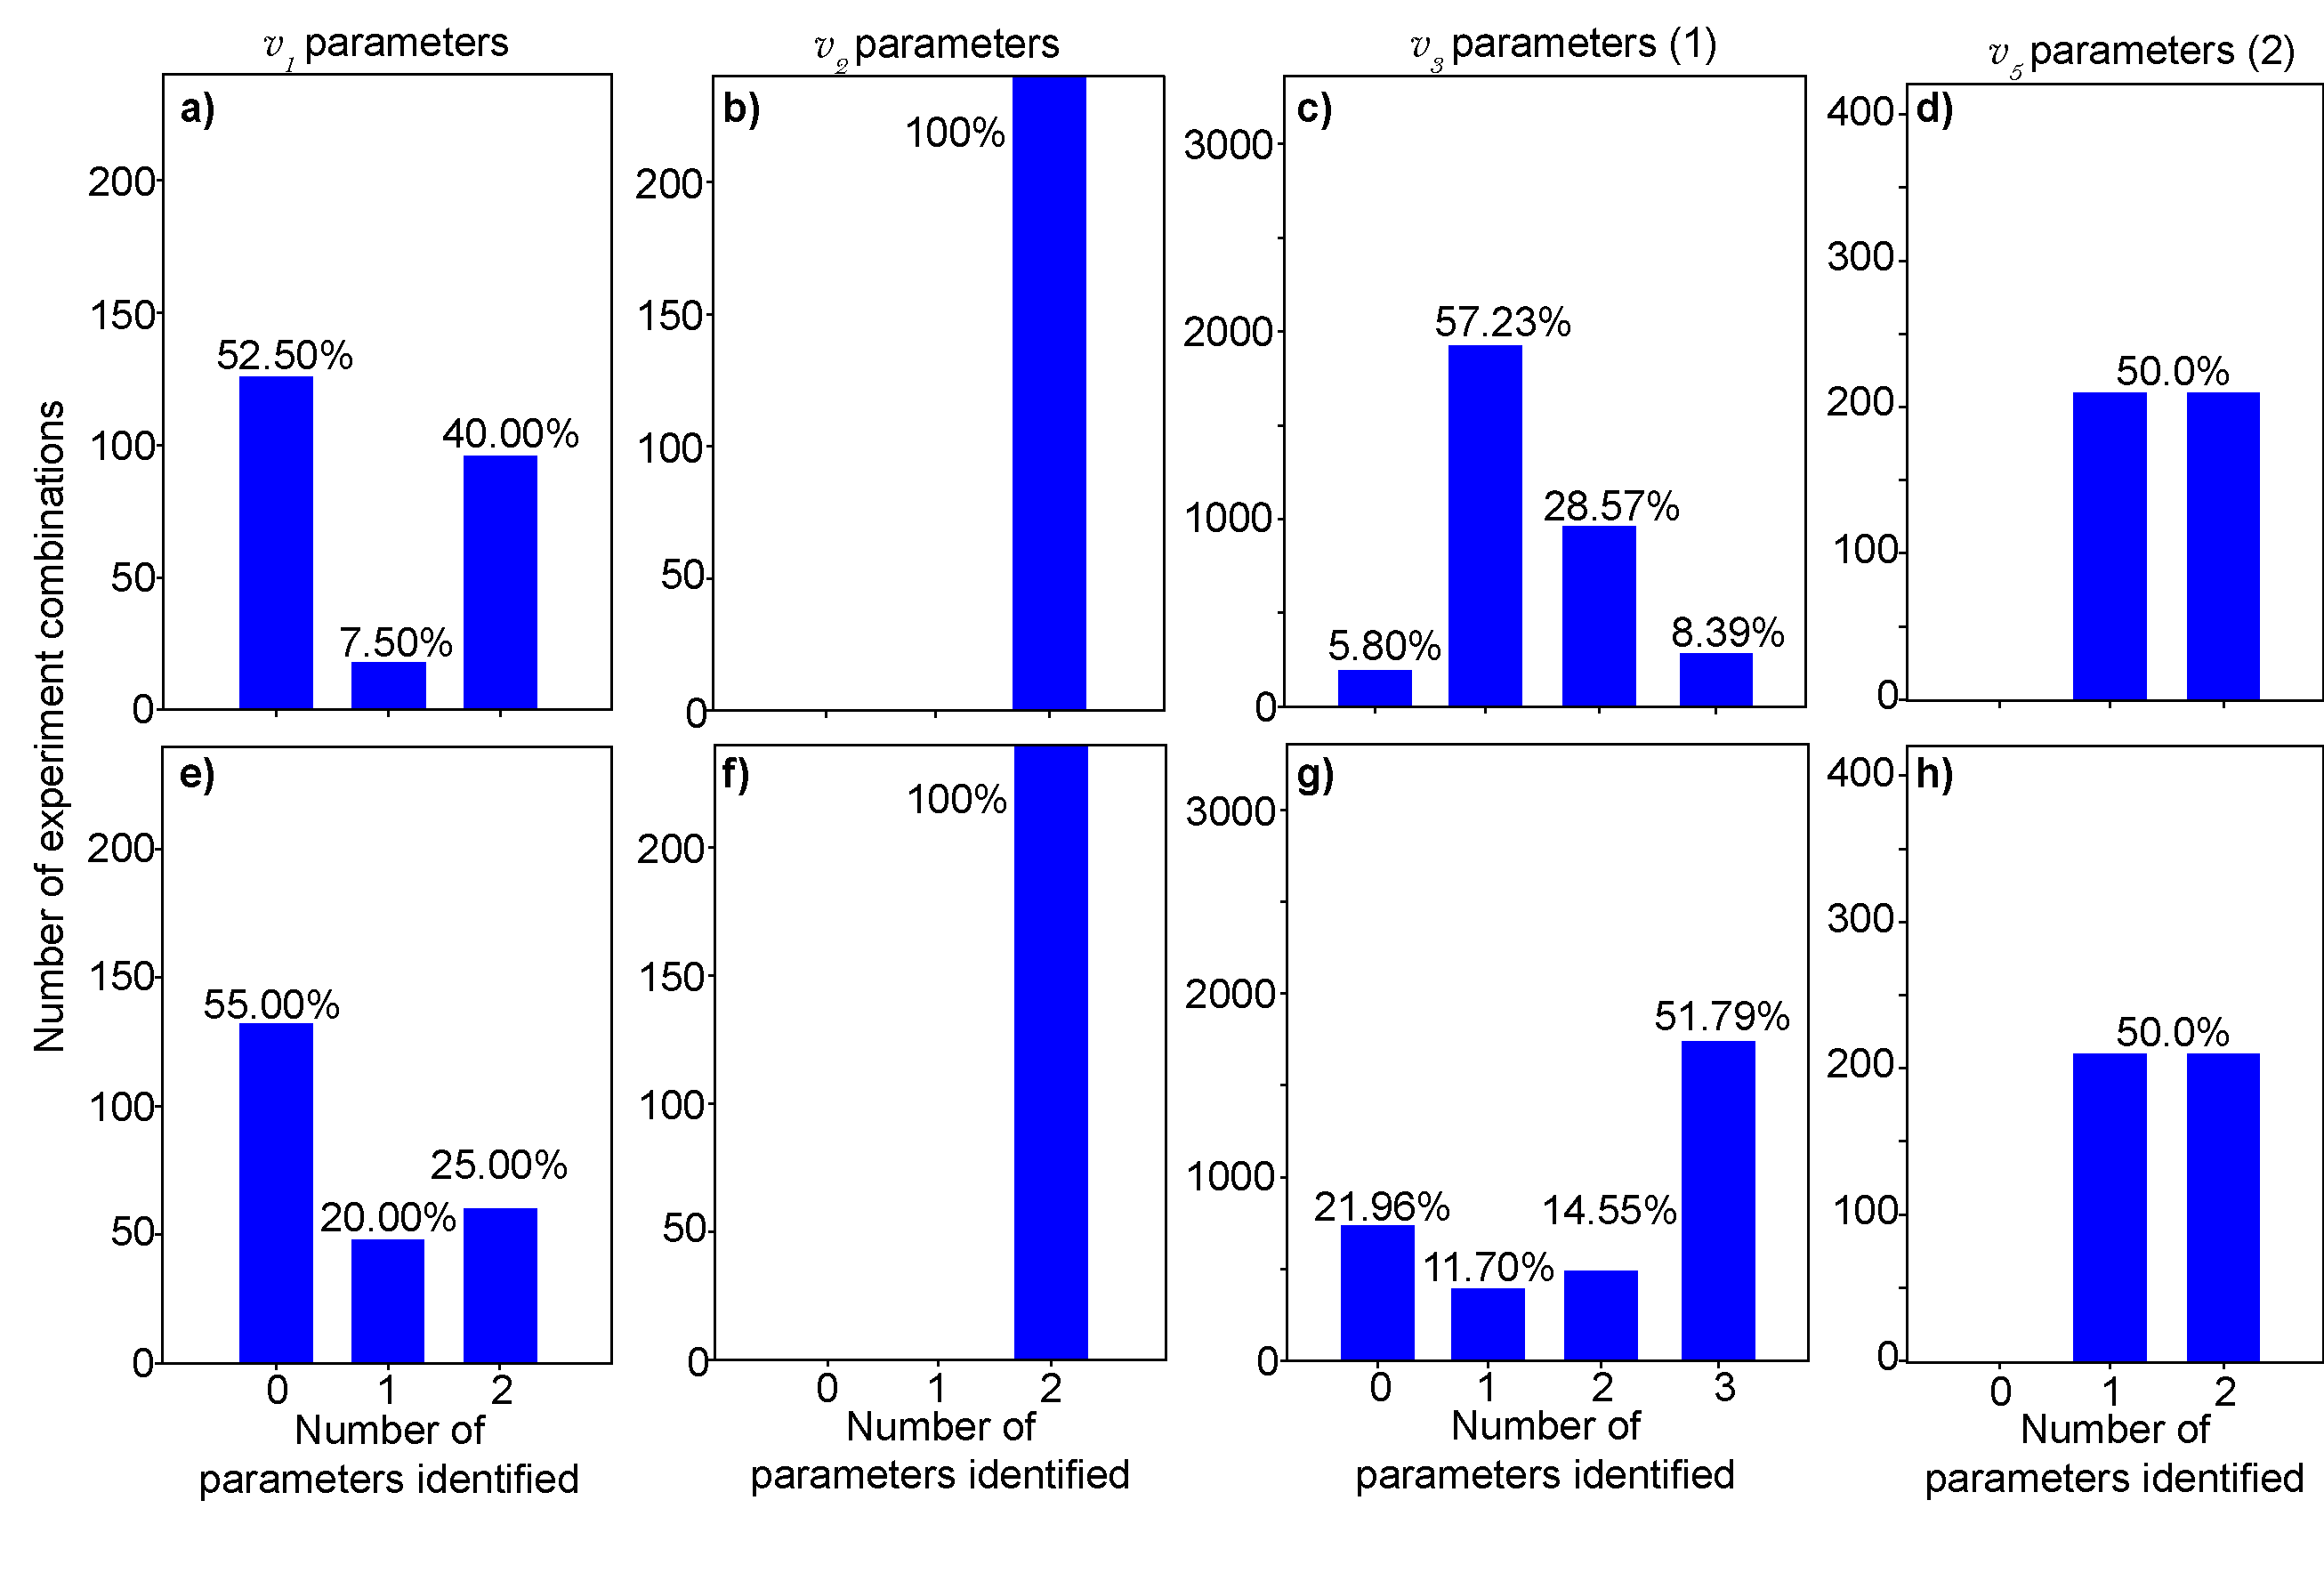
\includegraphics[width=1.0\textwidth,height=0.5\textheight,keepaspectratio]{figures/figure4/v1_V1max_v2_v3_1_v5_2_mwc_ck_data_utility}}
	\caption{Utility of experimental data combinations on the basis of their ability to identify the most number of parameters. Information is shown for parameters modeling fluxes a) $v_1$, b) $v_2$, c) $v_3$ and d) $v_5$. The total number of combinations of experimental data is shown in the vertical axis and the horizontal axis shows the total possible number of parameters that can be identified by data from combinations of a) two, b) two, c) three and d) two experiments. The percentages shown in the plots represent the fraction of the total combinations used to test identifiability of parameters for a given flux. A total of 240 data combinations are used for identifiability analysis for a) $v_1$ and b) $v_2$, 3360 combinations are used to practically identify c) $v_3$, and 420 combinations are used to analyze the identifiability of d) $v_5$. Section \ref{sec:experiments} provides more details on how the combinations of experimental data are generated.}\label{fig:data_utility}
\end{figure}	


\begin{figure}[!tbhp]
	\centering{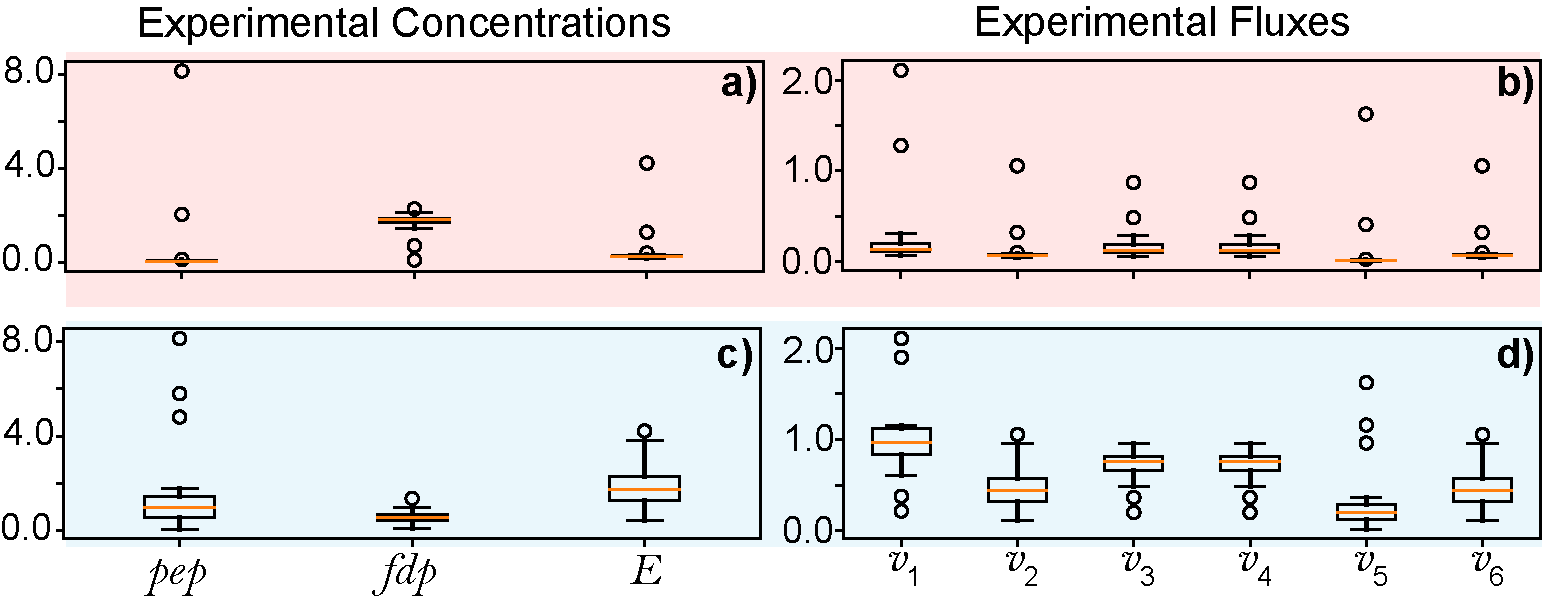
\includegraphics[width=1.0\textwidth,height=0.3\textheight, keepaspectratio]{figures/figure6/mwc_ck_experimental_data}}
	\caption{Variability in the metabolite concentrations and fluxes between different in silico experiments from which data is used for identifiability analysis. a) Metabolite (\textit{pep}, \textit{fdp}) and enzyme concentration (\textit{E}), and b) flux data ($v_1$, $v_2$, $v_3$, $v_4$, $v_5$ and $v_6$) are generated using the Monod-Wyman-Changeaux model for $v_3$. The Convenience Kientic rate law model is used for $v_3$ to generate in silico c) metabolite and enzyme concentration, and d) flux data through enzyme expression parameter and substrate concentration perturbations.}\label{fig:experimental_data_dist}
\end{figure}	

\begin{figure}[!tbhp]
	\centering{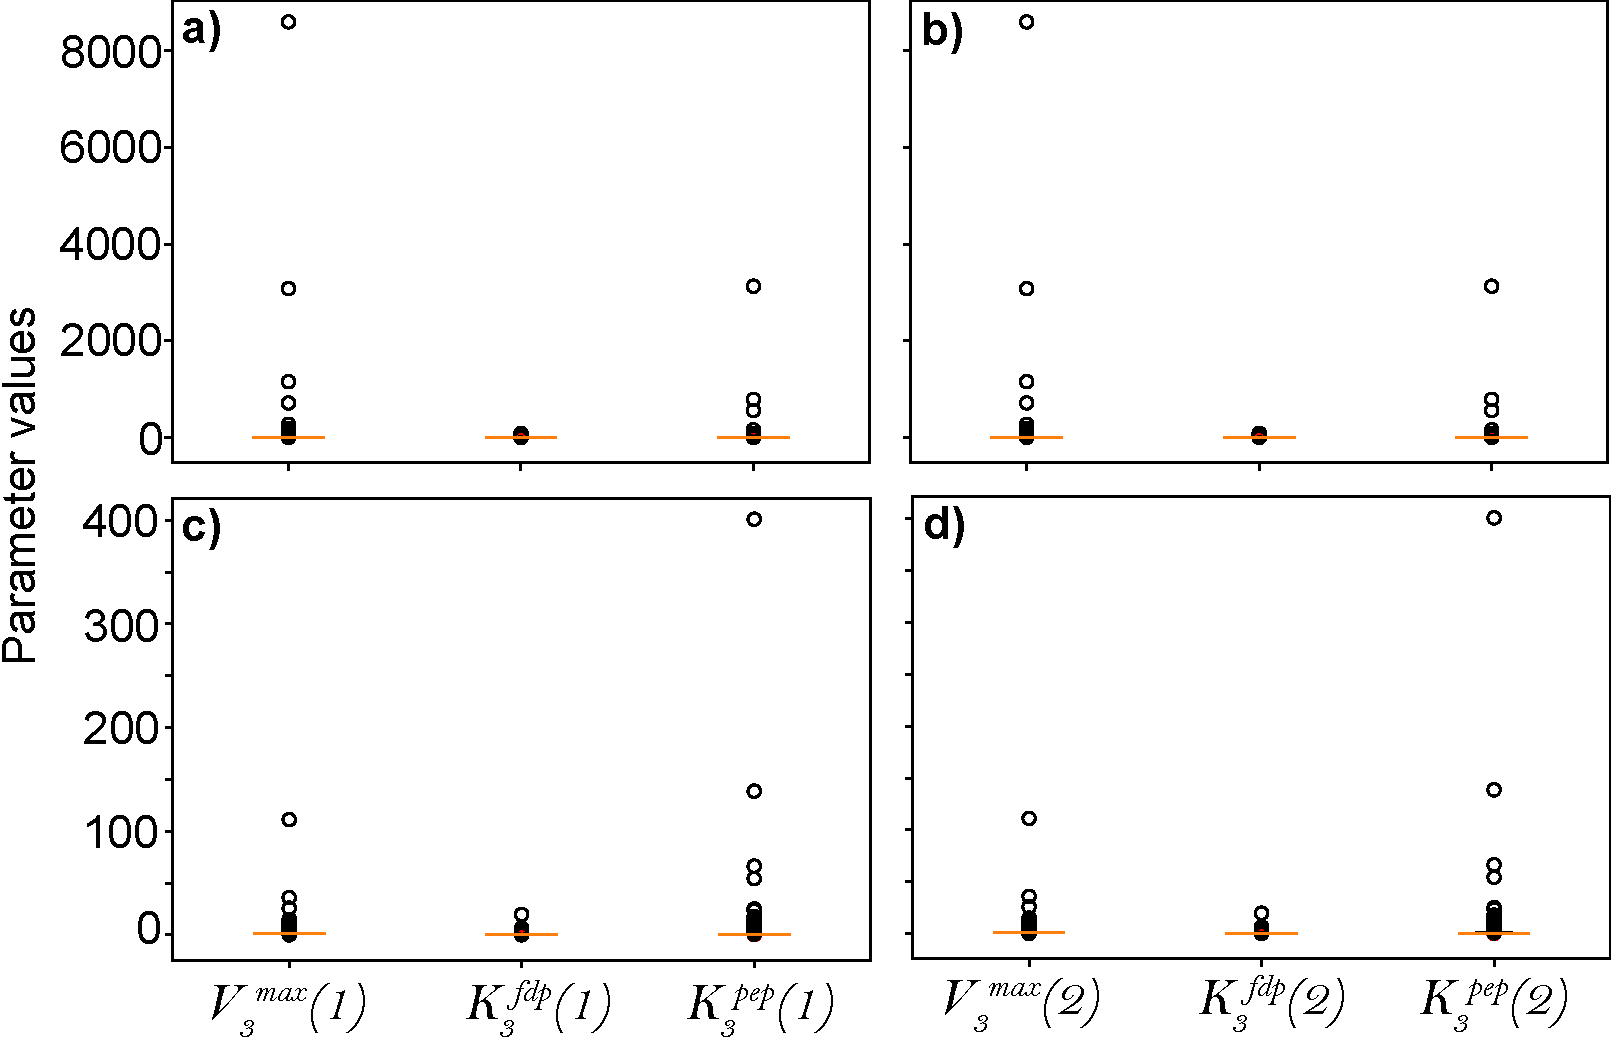
\includegraphics[width=1.0\textwidth,height=0.3\textheight, keepaspectratio]{figures/figure6/v3_1_2_ck_1_2_parameter_values}}
	\caption{Distribution of predicted parameter values when performing practical identifiability analysis using closed-form solutions for each parameter in flux $v_3$ when the a) and b) Monod-Wyman-Changeaux model for allosteric regulation for $v_3$ is used to generate data, c) and d) experimental data is generated using the Convenience Kinetic rate law model with activation for $v_3$. The left column corresponds to the first root for all three parameters: $V_3^{max}(1)$, $K_3^{fdp}(1)$ and $K_3^{pep}(1)$, and the second column corresponds to the second root of all three parameters in $v_3$: $V_3^{max}(2)$, $K_3^{fdp}(2)$ and $K_3^{pep}(2)$.}\label{fig:parameter_value_v3}
\end{figure}

\begin{figure}[!tbhp]
	\centering{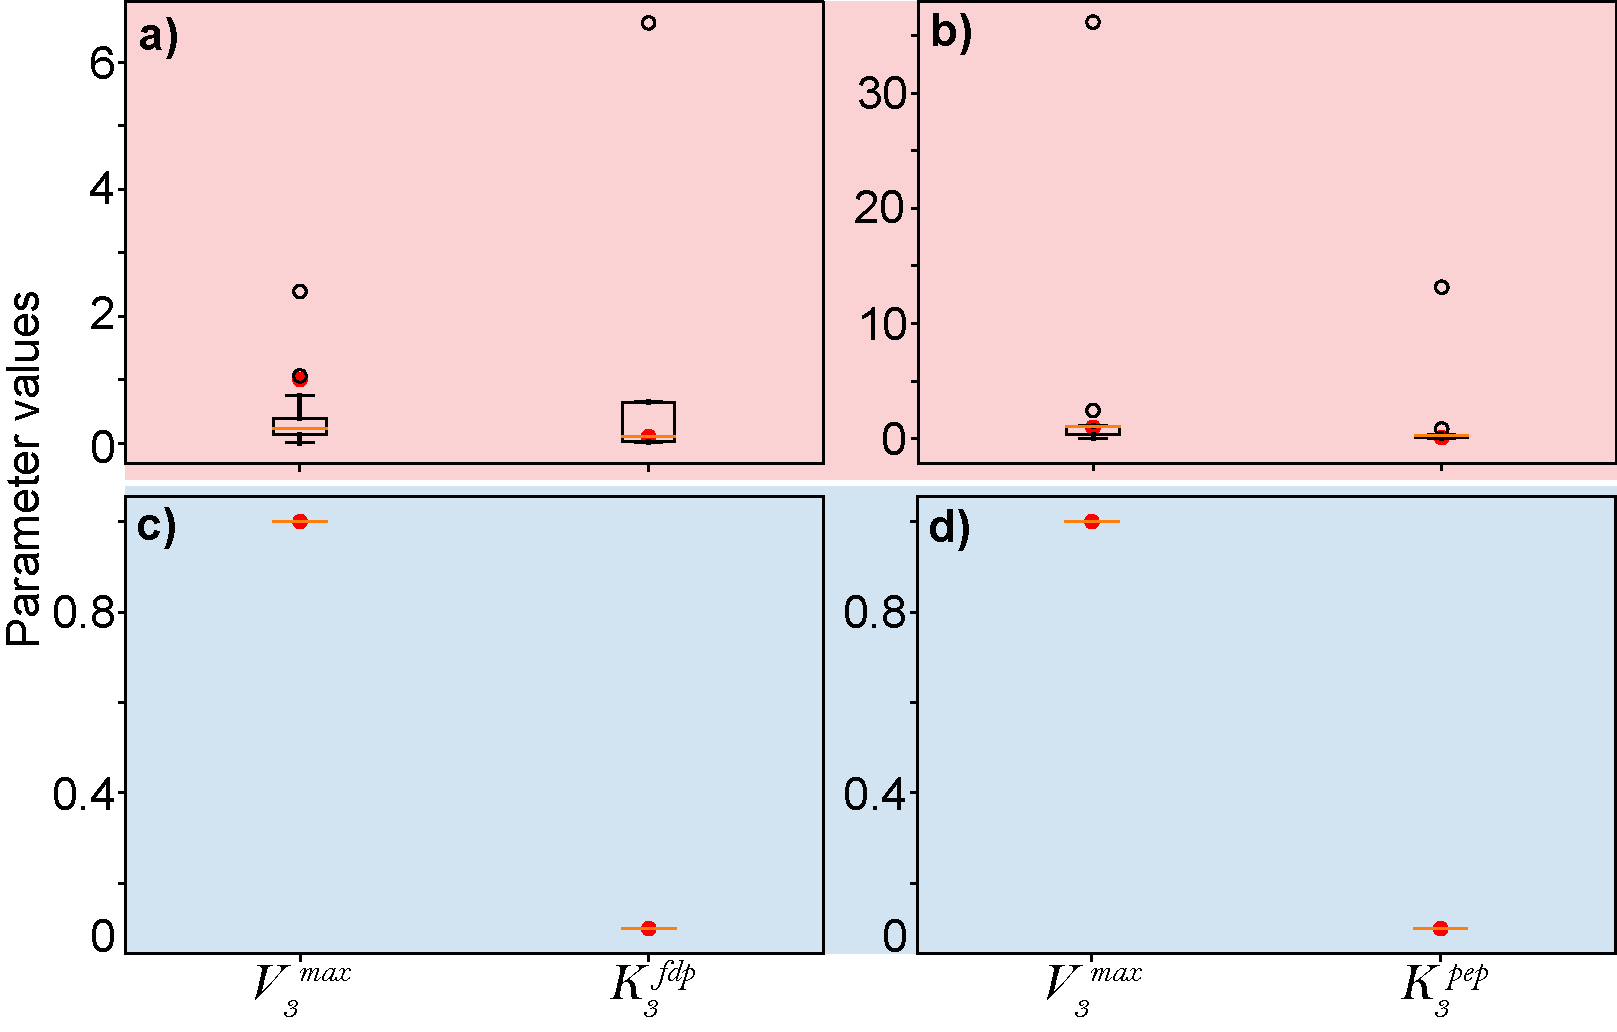
\includegraphics[width=1.0\textwidth,height=0.3\textheight, keepaspectratio]{figures/figure6/v3_var_1_2_ck_1_2_parameter_value}}
	\caption{Distribution of predicted parameter values when performing practical identifiability analysis using closed-form solutions for each parameter in flux $v_3$ when the a) and b) Monod-Wyman-Changeaux model for allosteric regulation for $v_3$ is used to generate data, c) and d) experimental data is generated using the Convenience Kinetic rate law model with activation for $v_3$. The left column shows the globally identifiable roots of $V_3^{max}$ and $K_3^{fdp}$ when $K_3^{pep}$ is held constant, and the right column shows the globally identifiable root of $V_3^{max}$ and $K_3^{pep}$ when $K_3^{fdp}$ is held constant.}\label{fig:parameter_value_v3_var}
\end{figure}	

%\begin{figure}[!tbhp]
	%\centering{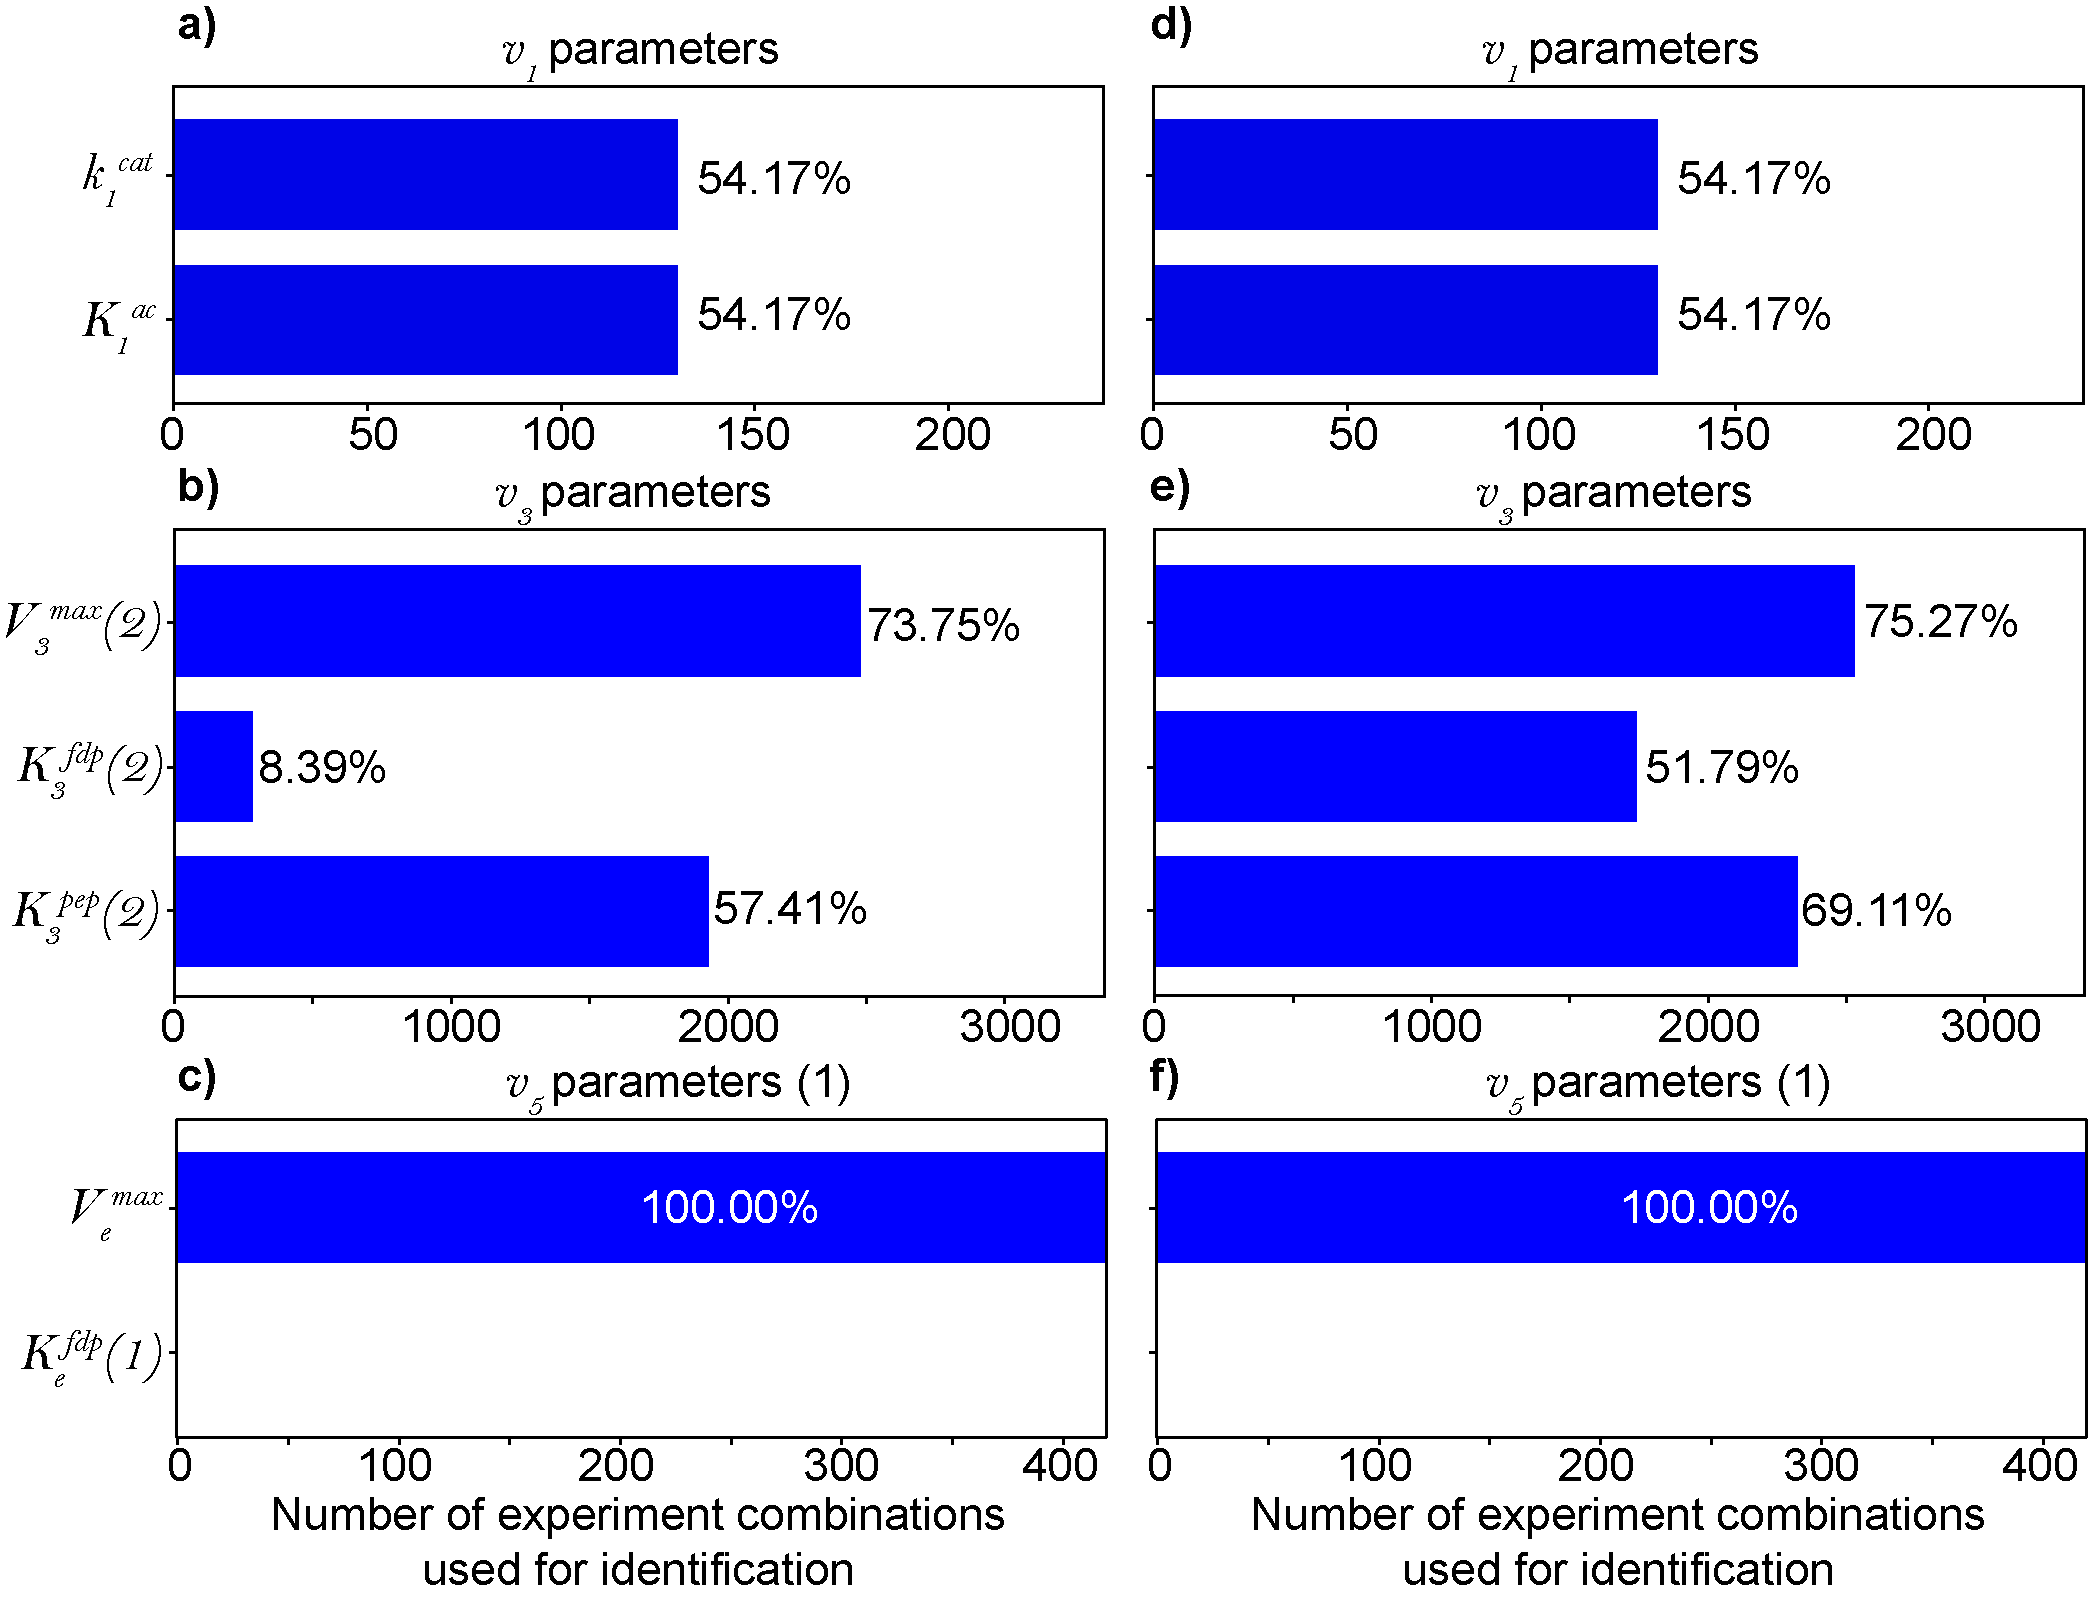
\includegraphics[width=1.0\textwidth,height=0.5\textheight, keepaspectratio]{figures/figure1/v1_k1cat_v3_2_v5_1_ident}}
	%\caption{The number of data combination from 21 different in silico experiments that can practically identify each parameter in fluxes a) and d) $v_1$, b) and e) $v_3$, and c) and f) $v_5$ when there is no noise in the input experimental data. The percentage of total combinations of experimental data used for analysis (240 for $v_1$ and $v_2$, 3360 for $v_3$ and 421 for $v_5$) that can identify each parameter is also specified. $v_1$, $v_2$ and $v_5$ require data from two experiments for analysis, and $v_3$ requires data from three experiments. Results for only one of the two possible roots are shown for $v_3$ and $K_e^{fdp}$ in $v_5$. The results obtained using data from the MWC model for $v_3$ are presented in the panels on the left hand side column and the panels on the right hand column show results obtained using data derived from the Convenience kinetics model for $v_3$.}\label{fig:ident_root2}
%\end{figure}

\begin{figure}[!tbhp]
	\centering{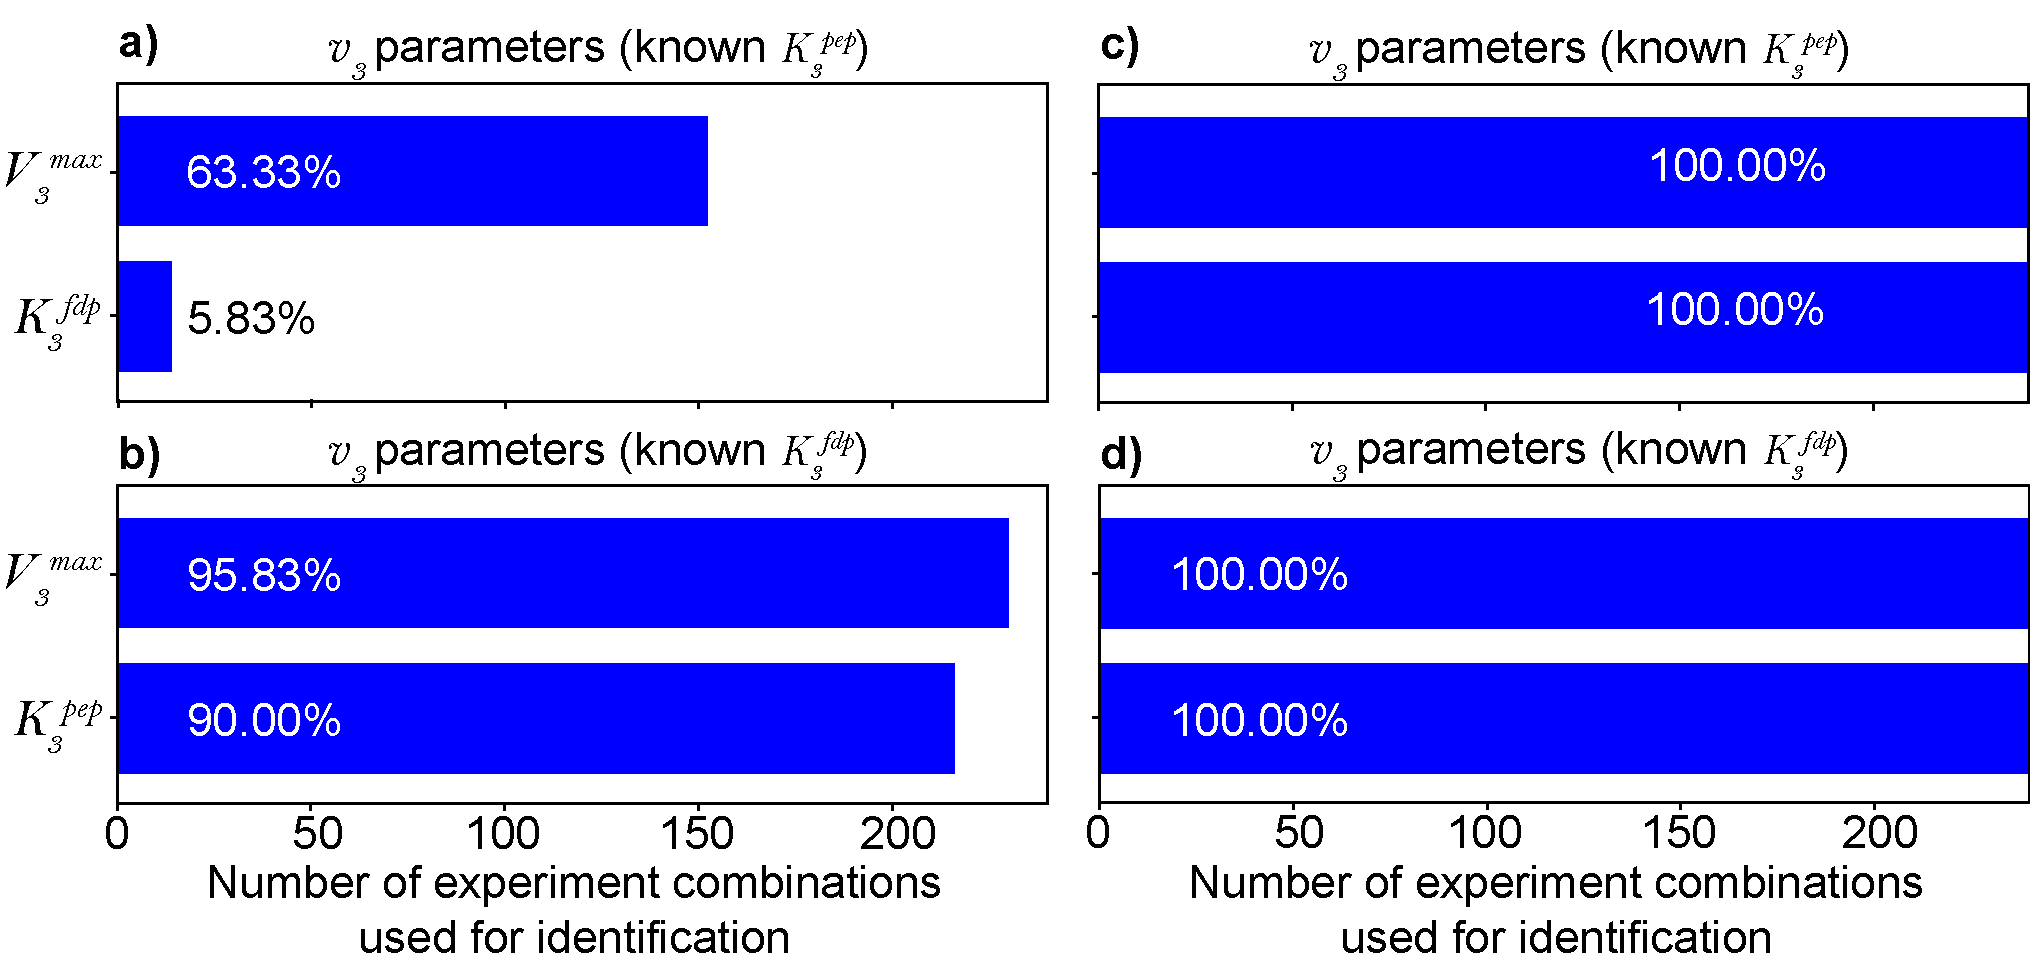
\includegraphics[width=1.0\textwidth,height=0.3\textheight, keepaspectratio]{figures/figure1/v3_1_2_mwc_ck_ident}}
	\caption{The number of data combination from 21 different in silico experiments that can practically identify each parameter in the convenience kinetic rate law model of flux $v_3$ when a) and c) $K_3^{pep}$ is held constant, and b) and d) $K_3^{fdp}$ is held constant. Results obtained using data from the MWC model for $v_3$ are presented in the panels on the left column and the panels on the right column show results obtained using data derived from the Convenience kinetics model for $v_3$. Note that all the identifiable parameters in the four panels are globally identifiable. The degree of identifiability of $V_3^{max}$ and $K_3^{pep}$ are higher when $K_3^{fdp}$ is held constant, than the degree of identifiability of $V_3^{max}$ and $K_3^{fdp}$ when $K_3^{pep}$ is held constant.}\label{fig:ident_v3_var}
\end{figure} 

\begin{figure}[!tbhp]
	\centering{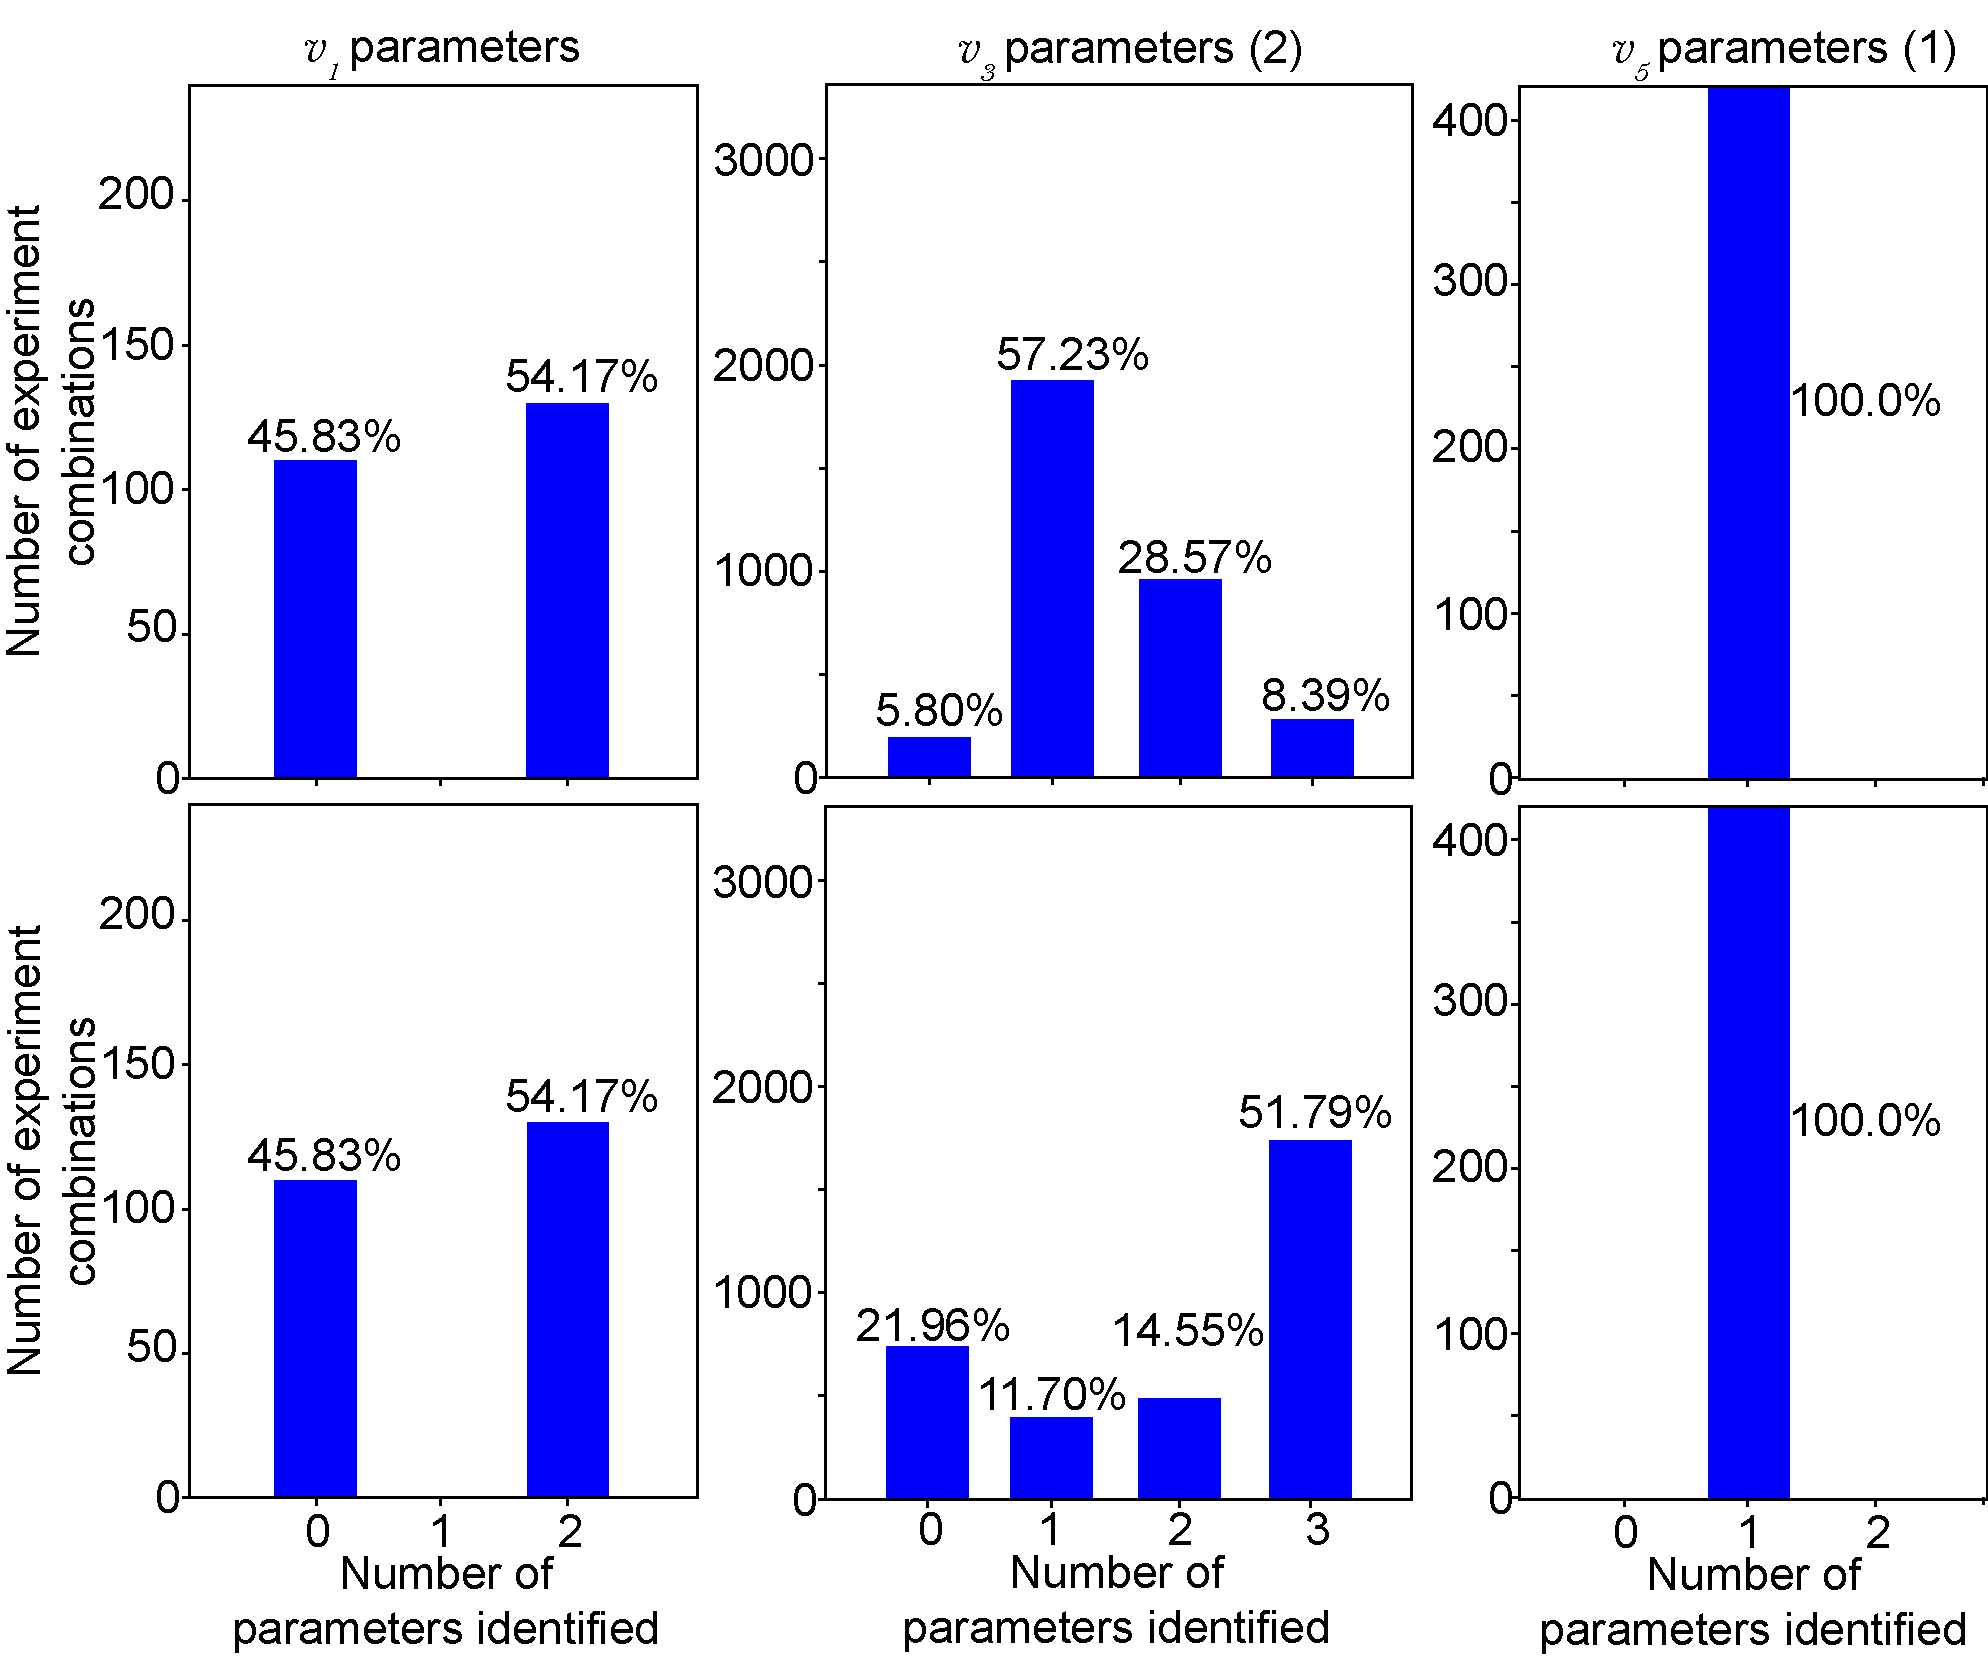
\includegraphics[width=1.0\textwidth,height=0.5\textheight, keepaspectratio]{figures/figure4/v1_k1cat_v3_2_v5_1_mwc_ck_data_utility}}
	\caption{Utility of experimental data combinations on the basis of their ability to identify the most number of parameters. Information is shown for parameters modeling fluxes a) $v_1$, b) $v_3$ and c) $v_5$. The total number of combinations of experiments is shown in the vertical axis, and the horizontal axis shows the maximum number of parameters that be identified using data from a combination of a) two, b) three and c) two experiments. The percentages shown in the plots represent the fraction of the total combinations used to test identifiability of parameters for a given flux. A total of 240 data combinations are used for identifiability analysis for a) $v_1$, \textcolor{red}{3360 combinations} are used to practically identify b) $v_3$, and 420 combinations are used to analyze the identifiability of c) $v_5$. Information processed based on the identifiability of a) $v_1$ in the presence of enzyme concentration data, b) the second root of parameters in $v_3$ and c) the first root of $K_e^{fdp}$ in $v_5$ are shown.}\label{fig:other_data_utility}
\end{figure}	

\begin{figure}[!tbhp]
	\centering{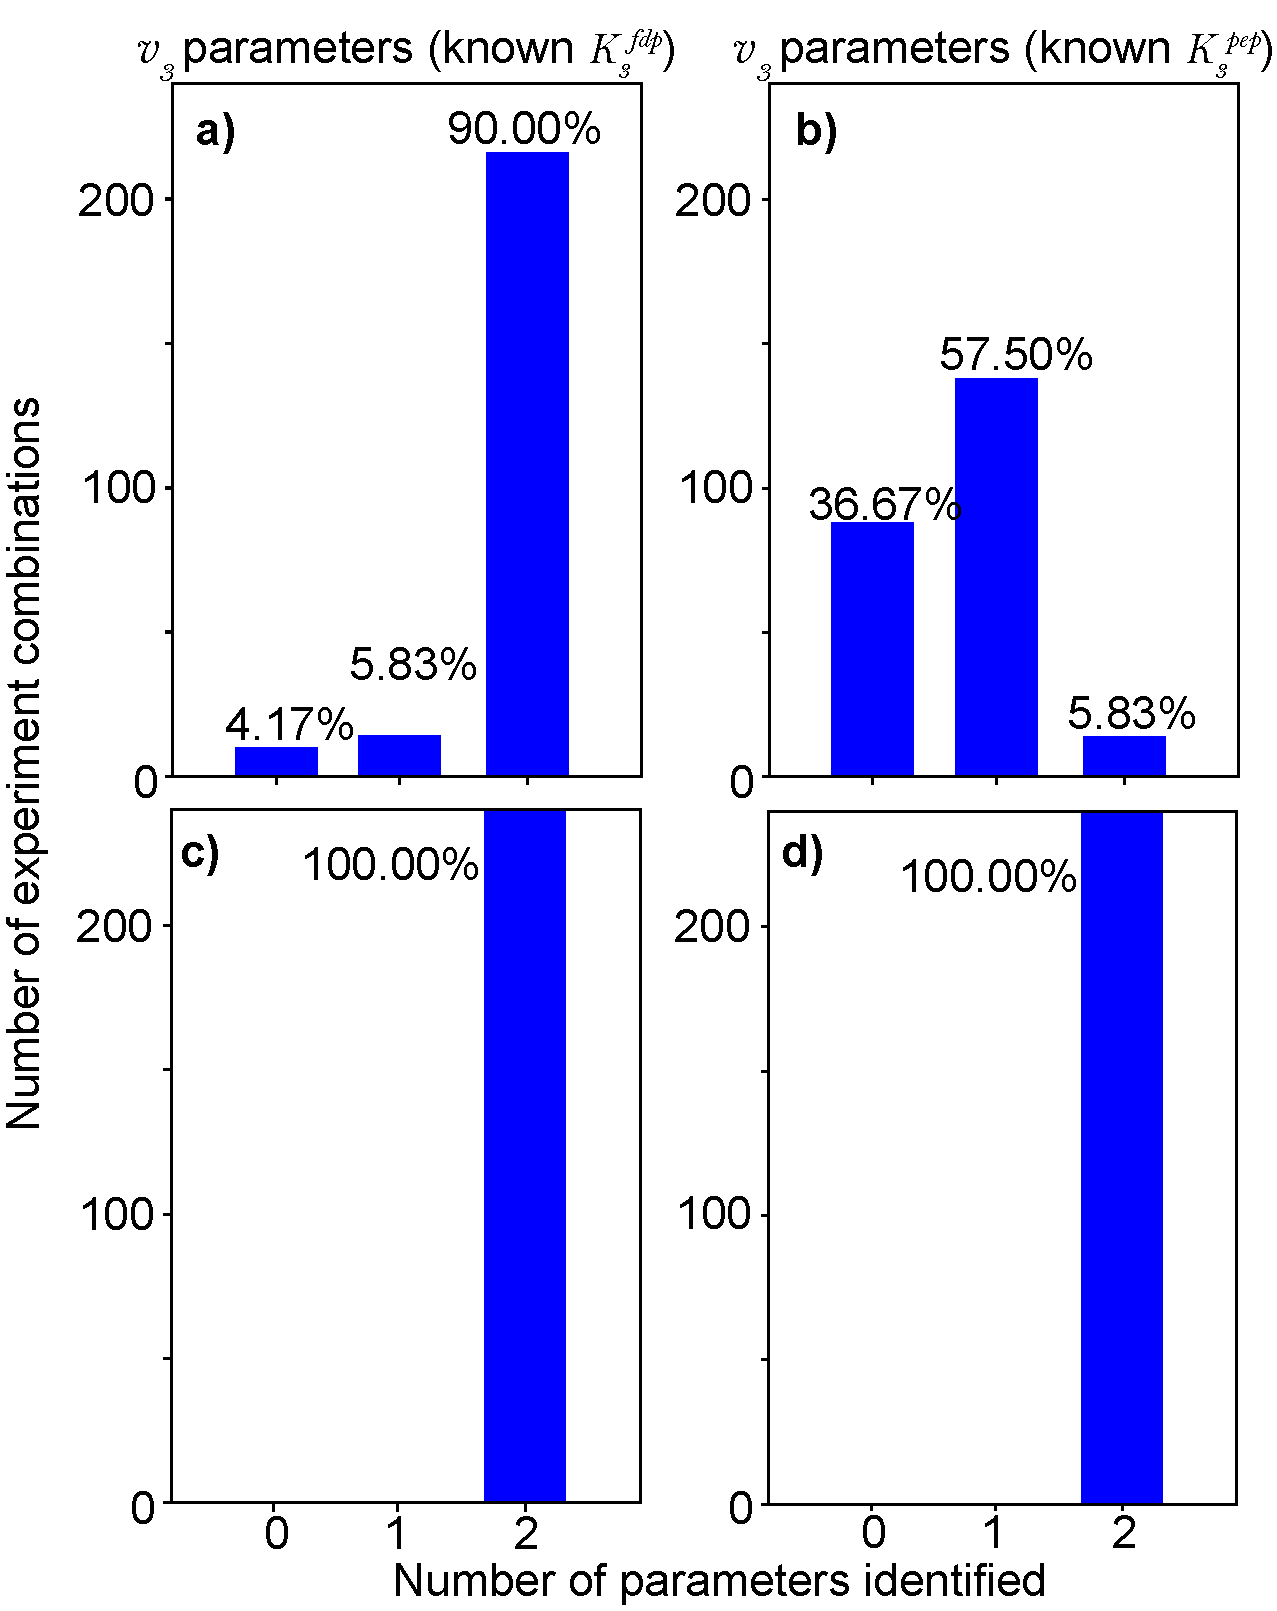
\includegraphics[width=1.0\textwidth,height=0.6\textheight, keepaspectratio]{figures/figure4/v3_var_1_2_mwc_ck_data_utility}}
	\caption{Utility of data from combinations of two different experiments for identifying two parameters in $v_3$ when a) $K_3^{pep}$ is held constant, and when b) $K_3^{fdp}$ is held constant. Notice that a significant number of combinations can identify both $V_3^{max}$ and $K_3^{pep}$ when $K_3^{fdp}$ is known and fixed. c and d data is from convenience kinetics model.}%\label{fig:figure2}
\end{figure}		

\begin{figure}[!tbhp]
	\centering{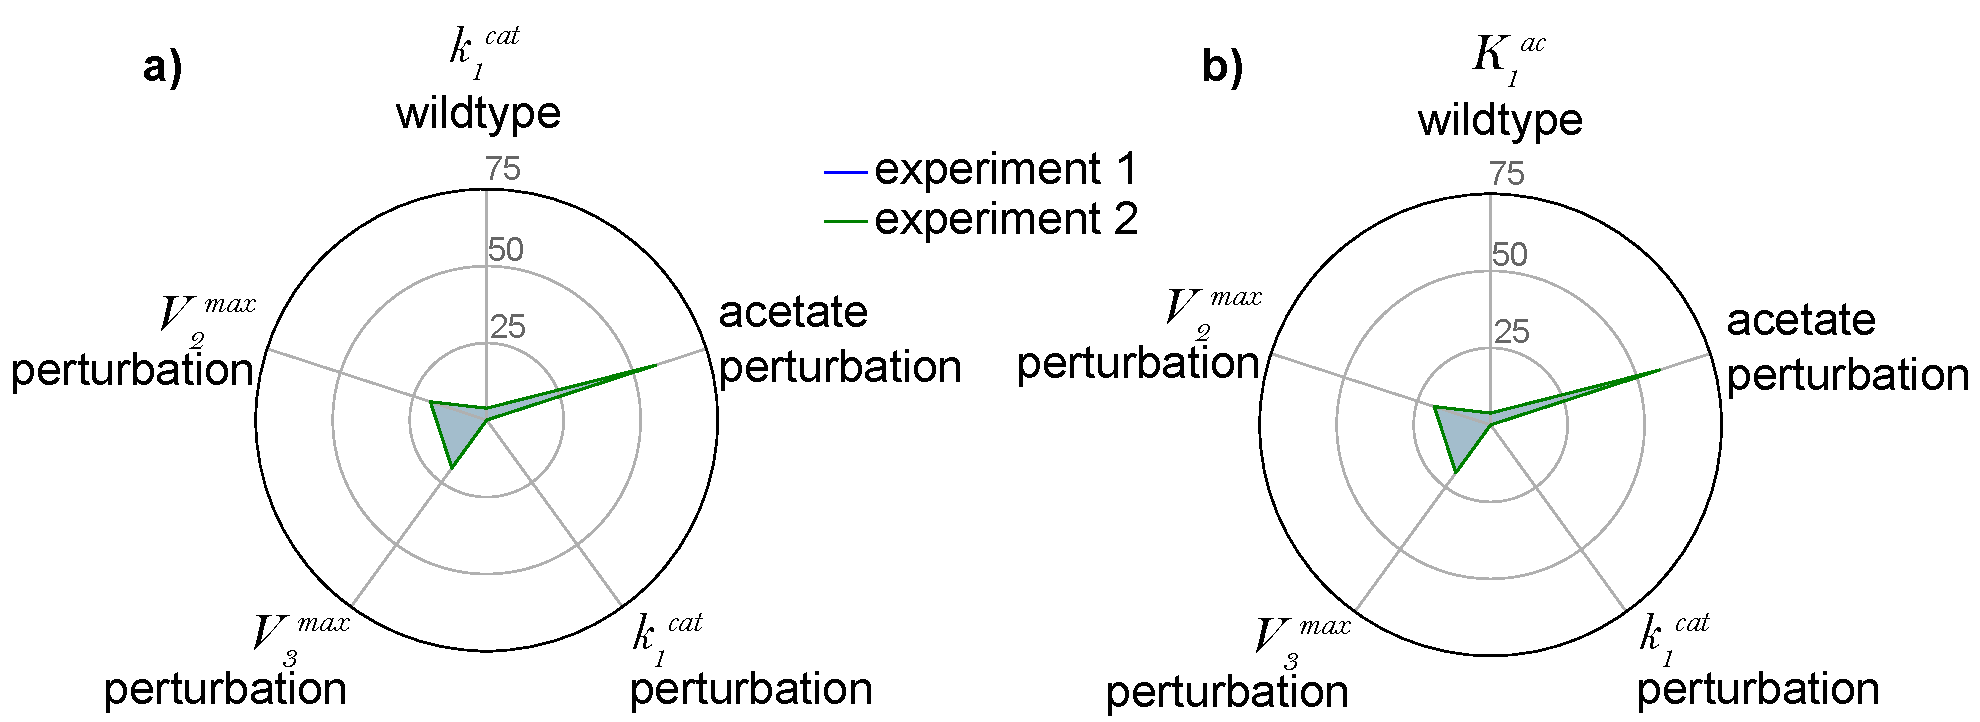
\includegraphics[width=1.0\textwidth,height=0.6\textheight, keepaspectratio]{figures/figure2/v1_k1cat_exp_info}}
	\caption{Contribution of different experiment types towards identification of a) $k_1^{cat}$ and b) $K_1^{ac}$ in $v_1$ based on using data from two different experiments. Data from MWC model.}%\label{fig:figure2}
\end{figure} 	

\begin{figure}[!tbhp]
	\centering{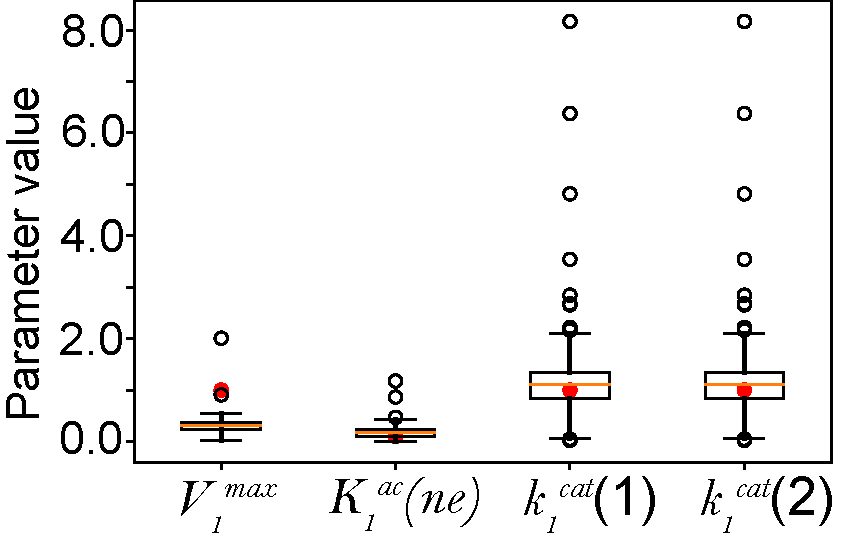
\includegraphics[width=1.0\textwidth,height=0.3\textheight, keepaspectratio]{figures/figure6/v1_v1max_k1cat_parameter_value}}
	\caption{Distribution of identified/estimated parameter values for flux $v_1$ from different experimental data combinations. The box plot of the estimated values of $V_1^{max}$ and $K_1^{ac}(ne)$ are juxtaposed with the box plots of the calculated values of $k_1^{cat}$ based on the estimated value of $V_1^{max}$ and the enzyme concentrations available from the two different experiments used to estimate $V_1^{max}$ and $K_1^{ac}(ne)$}\label{fig:parameter_value_v1_v1max_kcat}
\end{figure}	

\clearpage

\section{Supplementary Methods}
\subsection{Data for establishing parameter identifiability in kinetic model of gluconeogenesis}\label{sec:experiments}
Steady state information on the metabolome and the fluxome can be gathered under different physiological conditions. One way to alter the physiological conditions is to change the substrate concentration under which the cells grow. In the small metabolic network (Figure \ref{fig:network}), the acetate concentration plays the role of a substrate, and  determines the acetate uptake flux $v_1$ (Equation \ref{eq:flux1}). Thus, steady state metabolite concentrations and fluxes can be calculated under various acetate concentrations to form different experimental data combinations that measure cellular response to changes in the substrate concentration. 

Physiological changes can also be brought about by perturbing the expression levels for different enzymes within a metabolic network. The model of gluconeogenesis (Figure \ref{fig:network}) described in section \ref{sec:small-model} has three different fluxes ($v_1$, $v_2$ and $v_3$) whose enzyme expression parameters ($k_1^{cat}$, $V_2^{max}$ and $V_3^{max}$) can be perturbed to simulate the repression and over expression of the corresponding enzymes. Accordingly, in addition to measuring network responses to substrate perturbations, changes in steady state concentrations and fluxes can also be observed for enzyme expression perturbations. In total, based on the above discussion, we can perturb four different model parameters ($acetate$, $k_1^{cat}$, $V_2^{max}$ and $V_3^{max}$) to obtain experimental data in silico. The 21 different parameter values used to generate experimental data are given in Table \ref{tab:pval}. The box plots in Figure \ref{fig:experimental_data_dist} show the distribution in the in silico metabolite and enzyme concentration and flux data obtained from these experiments.

As described in section \ref{sec:ident} and Figure \ref{fig:ident-flowchart}b, the minimum number of experiments from which steady state data is required for identifying all the parameters of a given flux is determined by dimension $\mathbb{R}^p$ of the parameter space of a chosen flux $v_i$. For instance, the flux $v_2$ in the model described in section \ref{sec:small-model} has two parameters: $V_2^{max}$ and $K_2^{pep}$. Thus $\theta = \{V_2^{max}, K_2^{pep}\} \in \mathbb{R}^2$. So, steady state data from two distinct experiments is required for identifying $v_2$. Accordingly, multiple combinations of data generated from any two different experiments are used to test the identifiability of $v_2$. The total number of such possible combinations is 420 (21 x 20) from the 21 different experiments shown in Table \ref{tab:pval}. Assuming we also have data for the enzyme concentration $E$ in the expression for flux $v_1$ (Equation \ref{eq:flux1}), identifying the two parameters $k_1^{cat}$ and $K_1^{ac}$ ($\theta \in \mathbb{R}^2$) also requires steady state experimental data from two different experiments.

Similarly, for identifying $v_3$ that is described by three parameters ($\theta \in \mathbb{R}^3$), we need data from a combination of three different experiments. Based on the 21 experiments in Table \ref{tab:pval}, we have 7980 distinct combinations (21 x 20 x 19) of three experiments. However, it is important to note that not all of the either 420 combinations (for $v_1$ and $v_2$), or the 7980 combinations (for $v_3$), may be suitable for parameter estimation. Hence, the actual number of data combinations that can be used for practically identifying parameters in these fluxes would be smaller than the aforementioned numbers. Moreover, among the chosen smaller number of experimental data combinations, the methodology that we propose enables us to determine the number and nature of experimental data combinations, and consequently, the experiments that might allow for parameter identification, and subsequent parameter estimation.

\printbibliography

\end{document}

